\documentclass[12pt,a4paper]{report}
\usepackage[utf8]{inputenc}
\usepackage{amsmath}
\usepackage{amsfonts}
\usepackage{amssymb}
\usepackage{polski}
\usepackage{natbib}
\usepackage[hidelinks]{hyperref}
\usepackage[left=3cm,right=2.5cm,top=2.5cm,bottom=2.5cm]{geometry}
\linespread{1.3}
\author{Anita Kudaj}
\title{Matematyczne modele wykorzystywane w systemach rekomendacji.}

\newtheorem{df}{Definicja}
\newtheorem{tw}{Twierdzenie}
\newtheorem{dw}{Dowód}
\newtheorem{algorytm}{Algorytm}
\newtheorem{przyklad}{Przykład}
\newtheorem{metoda}{Metoda}
\newtheorem{problem}{Problem}

\usepackage{graphicx}
\usepackage{float}
\begin{document}


\begin{titlepage}
\begin{flushleft}
\end{flushleft}
\begin{center}
\textsc{{\huge Politechnika \L\'odzka}}
\end{center}
\bigskip
\bigskip
\begin{center}
\textsc{{\Large Wydzia\l\ Fizyki Technicznej, Informatyki i~Matematyki Stosowanej}}
\end{center}
\bigskip
\bigskip
\begin{Large}
Kierunek: Matematyka Stosowana\\
Specjalno\'s\'c: Analiza Danych w Biznesie i Logistyce
\\
\end{Large}
\bigskip
\bigskip
\noindent\hrulefill
\begin{center}
{\textbf{{\Large Matematyczne modele wykorzystywane w systemach rekomendacji.}}}
\end{center}
\begin{flushright}
{\large 
Anita Kudaj
\\
Nr albumu: 
220020
\\}
\end{flushright}
\noindent\hrulefill
\bigskip
\bigskip
\begin{center}
{\large Praca magisterska
\\napisana w Instytucie Matematyki Politechniki Łódzkiej\\ 
\bigskip
\bigskip
\bigskip
\bigskip
Promotor: dr, mgr inż. Piotr Kowalski
 }
\end{center}
\bigskip
\bigskip
\bigskip
\bigskip
\begin{center}
{\textsc{\large \L\'od\'z, ?????}}
\end{center}
\end{titlepage}


\tableofcontents

\chapter{Wstęp}
%TODO napiszemy na końcu
\chapter{Preliminaria} %teorie, definicje, twierdzenia z innych działów - potrzebne do zrozumienia pracy
\section{Elementy rachunku prawdopodobieństwa i statystyki}
Niech $F$ oznacza $\sigma$ - algebrę podzbiorów z przestrzeni $\Omega$ oraz niech $X$ oznacza funkcję rzeczywistą określoną na przestrzeni $\Omega$, to znaczy: %Krzyśko - Wykład z teorii pstwa
\begin{center}
$X: \Omega \longrightarrow \mathbb{R}$.
\end{center}
\begin{df}\textbf{Zmienna losowa}%Krzyśko - Wykład z teorii pstwa
\\Zmienną losową nazywamy funkcję $X$, która jest $F$ - mierzalna, to znaczy jeżeli dla każdego $a\in\mathbb{R}$ zachodzi:
\begin{center}
$\{\omega : X(\omega) < a\} = X^{-1}((-\infty,a))\in F$, 
\end{center}
gdzie $X^{-1}$ jest operacją przeciwobrazu zbioru przez funkcję $X$.
\end{df}

\begin{df}\textbf{Kowariancja}
\\Kowariancją zmiennych losowych $X,Y$ nazywamy liczbę:
\begin{center}
$Cov(X,Y) = E[(X-E(X))(Y-E(Y))]$,
\end{center}
gdzie $E(X)$ oznacza wartość oczekiwaną zmiennej losowej $X$.
\end{df}
\begin{df}\textbf{Odchylenie standardowe}
\\Wariancją zmiennej losowej $X$ nazywamy liczbę:
\begin{center}
$Var(X)=E([X-E(X)]^2)$,
\end{center}
jeżeli po prawej stronie równości wartość oczekiwana istnieje. 
\\Odchyleniem standardowym zmiennej losowej $X$ nazywamy liczbę:
\begin{center}
$\sigma(X)=\sqrt{Var(X)}$.
\end{center}
\end{df}
\begin{df}\textbf{Współczynnik korelacja}
\\Współczynnikiem korelacji nazywamy charakterystykę ilościową stopnia zależności dwóch zmiennych losowych $X$ i $Y$ zdefiniowaną następująco:
\begin{center}
$\rho(x,Y) = \frac{Cov(X,Y)}{\sigma(X)\sigma(Y)}$.
\end{center}
\end{df}
W statystyce do przedstawienia poziomu zależności liniowej między dwoma zmiennymi losowymi używamy Współczynnika Korelacji Pearsona.
\begin{df}\textbf{Współczynnik Korelacji Pearsona}
\\Niech $X,Y \in \mathbb{R}^n$ będą zmiennymi losowymi o rozkładach ciągłych oraz niech $x_k$, $y_k$, gdzie $k\in\{1,...,n\}$ oznaczają wartości prób losowych tych zmiennych. 
\\Przez $\overline{x}$ i $\overline{y}$ oznaczmy:
\begin{center}
$\overline{x}=\frac{1}{n} \sum_{k=1}^n x_k$,
\\$\overline{y}=\frac{1}{n} \sum_{k=1}^n y_k$.
\end{center}
Wówczas Współczynnikiem Korelacji Pearsona nazywamy:
\begin{center}
$\rho(X,Y) = \frac{\sum_{k=1}^n(x_k - \overline{x})(y_k - \overline{y})}{\sqrt{\sum_{k=1}^n(x_k - \overline{x})^2} \sqrt{\sum_{k=1}^n(y_k - \overline{y})^2 }}$.
\end{center}
\end{df}
\section{Elementy algebry liniowej}
\begin{df}\textbf{Iloczyn skalarny}
\\Niech $U$ oznacza przestrzeń liniową nad ciałem $\mathbb{R}$. Iloczynem skalarnym nazywamy formę dwuliniową 
\begin{center}
$d: U \times U \longrightarrow \mathbb{R}$,
\end{center}
gdy:
\begin{itemize}
\item dla każdego $u \in U$ zachodzi:
\begin{center}
$d (u,u) \geq 0$
\end{center}
\item jest symetryczna, oznacza to, że dla dowolnych $u, v \in U$ zachodzi:
\begin{center}
$d(u,v)=d(v,u)$
\end{center}
\item $\d(u,u)=0 \Leftrightarrow u = \Theta_{U}$
\end{itemize}
Przestrzeń liniową $U$ nad ciałem liczb rzeczywistych z iloczynem skalarnym 
\\$d: U \times U \longrightarrow \mathbb{R}$ nazywamy przestrzenią euklidesową.
\end{df}
%Larose -> odkrywanie wiedzy z danych
\begin{df} \textbf{Miara odległości}
\\Miarą odległości (funkcją odległości) nazywamy rzeczywistą funkcję $d$, która dla każdego $x, y, x \in \mathbb{R}^n$ spełnia warunki:
\begin{itemize}
\item $d(x,y)\geq 0$ 
\item $d(x,y) = 0 \Leftrightarrow x = y$ 
\item $d(x,y) = d(y,x)$
\item $d(x,y) + d(y,z) \geq d(x,z)$
\end{itemize}
\end{df}

\begin{df}\textbf{Odległość euklidesowa} %Spodzieja S.: Wstęp do analizy matematycznej funkcje jednej zmiennej.
\\Niech $(x_1,x_2,...,x_n) \in \mathbb{R}^n $.
Normą x nazywamy:
\begin{center}
$||x|| = \sqrt{x_{1}^{2} + ... + x_{n}^{2}}$.
\end{center}
Jeśli $x,y \in \mathbb{R}^n $ to liczbę:
$||x-y||$ nazywamy odległością euklidesową punktów $x$ i $y$, gdzie:
\begin{center}
$(x-y) = (x_1-y_1,...,x_n-y_n)$.
\end{center}
\end{df}
\begin{df}\textbf{Odległość kosinusowa} %https://pqstat.pl/?mod_f=macpod
\\Niech $x,y \in \mathbb{R}^n $ (x,y są n-wymiarowymi wektorami). Odległością kosinusową nazywamy:
\begin{center}
$d(x,y) = 1 - sim (x,y)$, 
\end{center}
gdzie $sim (x,y)$ to współczynnik podobieństwa wektorów $x$ i $y$:
\begin{center}
$sim (x,y) = \frac{x \cdot y}{|x||y|}$,
\end{center}
zatem
\begin{center}
$sim (x,y) = \frac{\sum_{k=1}^n x_k y_k}{\sqrt{\sum_{k=1}^n x_k}\sqrt{\sum_{k=1}^n y_k}}$.
\end{center}
\end{df}
\begin{df}\textbf{Macierz transponowana}%Banaszak "Elementy algebry liniowej cz.1"
\\Niech dana będzie macierz $A \in M_{m,n}(K)$ o $n$ kolumnach i $m$ wierszach:
\begin{center}
$ A= \left[
        \begin{array}{cccc}
         a_{11} & a_{12} & \cdots & a_{1n}\\
         a_{21} & a_{22} & \cdots & a_{2n}\\
         \vdots & \vdots & \ddots & \vdots\\
         a_{m1} & a_{m2} & \cdots & a_{mn}\\
         \end{array}
      \right]
      \qquad $.
\end{center}
Macierzą transponowaną nazywamy macierz $A^T \in M_{n,m}(K)$:
\begin{center}
$ A^T= \left[
        \begin{array}{cccc}
         a_{11} & a_{21} & \cdots & a_{m1}\\
         a_{12} & a_{22} & \cdots & a_{m2}\\
         \vdots & \vdots & \ddots & \vdots\\
         a_{1n} & a_{2n} & \cdots & a_{mn}\\
         \end{array}
      \right]
      \qquad $.
\end{center}
\end{df}
\begin{tw}\textbf{Własności transpozycji macierzy}
\\Niech $A$ i $B$ będą macierzami o współczynnikach z $K$ oraz niech posiadają tyle kolumn i wierszy, że operacje występujące powyżej są określone. Niech $\lambda \in K$.
\\Zachodzą następujące równości:
\begin{itemize}
\item $(A^T)^T = A$,
\item $(A + B)^T = A^T + B^T$,
\item $(\lambda A)^T = \lambda A^T$,
\item $(AB)^T = B^T A^T$.
\end{itemize}
\end{tw}
\begin{df}\textbf{Macierz ortogonalna}
\\Macierzą ortogonalną nazywamy macierz kwadratową $A \in M_{n,n}(\mathbb{R})$ spełniającą nierówność:
\begin{center}
$A^T \cdot A = A\cdot A^T = I_n$,
\end{center}
gdzie $A^T$ oznacza macierz transponowaną względem $A$, natomiast $I_n$ oznacza macierz jednostkową.
\end{df}

\begin{df}\textbf{Macierz diagonalna}
\\Macierzą diagonalną nazywamy macierz $A\in M_{n,n}(K)$ taką, że:
\begin{center}
$A = (a_{ij})$ dla $i,j=1,2,...,n$ 
\\oraz 
\\$a_{ij} = 0$ gdy $i\neq j$.
\end{center}
\end{df}

\begin{df}\textbf{Macierz nieosobliwa}
\\Macierzą nieosobliwą nazywamy macierz kwadratową $A \in M_{n,n}(K)$, jeżeli istnieje macierz $B \in M_{n,n}(K)$ taka, że:
\begin{center}
$A \cdot B = B \cdot A = I_n$,
\end{center}
gdzie $I_n$ jest macierzą jednostkową.
\end{df}
\begin{df}\textbf{Macierz osobliwa}
\\Macierzą osobliwą nazywamy macierz kwadratową $A \in M_{n,n}(K)$, której wyznacznik jest równy zero.
\end{df}
\begin{df}\textbf{Rozkład wartości osobliwych}
\\Rozkładem wartości osobliwych nad $\mathbb{R}$ nazywamy przedstawienie macierzy $A$ w postaci:
\begin{center}
$A = \mathbb{U}\sum \mathbb{V}^T$,
\end{center}
gdzie $\mathbb{U}$ i $\mathbb{V}$ są macierzami ortogonalnymi. Natomiast $\sum$ jest macierzą diagonalną, która zawiera kolejne wartości osobliwe.
\end{df}

\begin{df}\textbf{?Macierz odwrotna}
\end{df}

\begin{df}\textbf{Ślad macierzy}
\\Śladem macierzy  $A\in M_{n,n}(K)$ nazywamy wielkość:
\begin{center}
$tr(A) = \sum_{i=1}^n a_{ii} = a_{11} + a_{22} + \cdots + a_{nn}$.
\end{center}
\end{df}
\begin{df}\textbf{Rząd macierzy}%Banaszak "Elementy algebry liniowej cz.1"
\\Rzędem macierzy nazywamy liczbę wiodących jedynek w dowolnej postaci zredukowanej macierzy. Rząd macierzy A oznaczamy symbolem $rz A$ lub $R(A)$.
\end{df}
Rząd macierzy wyznacza maksymalną wektorów niezależnych, które są kolumnami lub wierszami tej macierzy.
\begin{df}\textbf{?Zakres macierzy}
\end{df}
\begin{df}\textbf{?Jądro macierzy}
\end{df}
\begin{df}\textbf{Przestrzeń generowana przez układ wektorów}
\\Przestrzenią generowaną przez układ wektorów $X$ nazywamy zbór wszystkich kombinacji linowych skończonych podukładów $X$.
\\Oznaczamy ją symbolem $span(X)$ i definiujemy ją następująco:
\begin{center}
$span(X) := \{\sum_{i=1}^n a_i x_i : (\forall_{i\in [1;n]\cap \mathbb{N}} a_i \in \mathbb{K}) \wedge (\forall_{i\in [1;n]\cap \mathbb{N}} x_i \in \mathbb{X}) \wedge n \in \mathbb{N}\}$,
\end{center}
gdzie $X = (x_i)_{i=1}^n$ jest układem wektorów przestrzeni wektorowej $\mathbb{V}$ nad ciałem $\mathbb{K}$.
\end{df}

\chapter{Eksploracja danych w systemach rekomendujących}
Większość systemów rekomendujących opiera swój rdzeń na algorytmach, które możemy rozumieć jako konkretne przypadki technik eksploracji danych. 
\\Proces eksploracji danych składa się zazwyczaj z trzech kroków:
\begin{enumerate}
\item Preprocesing Danych,
\item Analiza Danych,
\item Interpretacja Wyników.
\end{enumerate}
W tym rozdziale zostaną przeanalizowane najważniejsze i najczęściej używane w regułach rekomendujących metody. Zaczniemy od miar podobieństw i redukcji wymiaru. W kolejnym etapie spojrzymy na metody klasyfikacji, grupowania i regresji, aby zakończyć interpretacją wyników i oceną błędów obliczeń.
\section{Preprocesing danych}
Przed przystąpieniem do kroku analizy dane wymagają przygotowania: wyczyszczenia, przefiltrowania, transformacji. Dopiero tak przygotowane dane mogą zostać poddane zadaniom uczenia maszynowego. W tej sekcji zostaną przedstawione problemy, które spotkamy przy tworzeniu reguł rekomendujących.
\subsection{Miary podobieństwa}
W systemach rekomendujących, jak filtrowanie kolaboratywne bardzo częstym podejściem jest używanie metod klasyfikacji i grupowania. Metody te bardzo ściśle opierają się na obliczaniu podobieństwach i odległości.
\\Najprostszym i jednocześnie najczęściej używanym podejściem jest tu \textbf{Odległość Euklidesowa}:
\begin{center}
$d(x,y) = \sqrt{\sum_{k=1}^n (x_k-y_k)^2}$, 
\end{center}
gdzie $n$ oznacza liczbę atrybutów elementów $x$ i $y$ przy czym $x_k$ oznacza k-ty atrybut elementu $x$. 
\\Innym przykładem jest \textbf{Odległość Minkowkskiego}, która jest uogólnioną wersją Odległości Euklidesowej:
\begin{center}
$d(x,y) = (\sum_{k=1}^n|x_k-y_k|^r)^{\frac{1}{r}}$.
\end{center}
W zależności od wartości stopnia odległości $r$ Odległość Minkowkskiego przyjmuje konkretne nazwy:
\begin{itemize}
\item $r=1$ - Odległość Manhatan (norma $L_1$),
\item $r=2$ - wspomniana wcześniej Odległość Euklidesowa,
\item $r \longrightarrow \infty $ - supremum ( norma $L_{max}$, norma $L_{\infty}$). 
\end{itemize}
Kolejnym podejściem, gdzie poszczególne elementy są postrzegane jako $n$ - wymiarowe wektory, a podobieństwo między nimi jest obliczane na podstawie konta, który tworzą jest \textbf{podobieństwo kosinusów}:
\begin{center}
$cos(x_u, x_v) = \frac{x_u^{T}x_v}{||x_u|| ||x_v||}$,
\end{center}
gdzie $x_u$ i $x_v$ oznaczają wektory preferencji użytkowników $u$ oraz $v$.
\\Inną miarą jest \textbf{Korelacja Pearsona}, zdefiniowana następująco:
\begin{center}
$\rho(u,v) = \frac{\sum_{i\in I_{uv}}(r_{ui}-\overline{r}_u)(r_{vi}-\overline{r}_v)}{\sqrt{\sum_{i\in I_{uv}}(r_{ui}-\overline{r}_u)^2 \sum_{i\in I_{uv}}(r_{vi}-\overline{r}_v)^2}}$
\end{center}
$I_{uv}$ oznacza w tym przypadku zbiór elementów, które zostały ocenione przez użytkownika $u$ i użytkownika $v$, $r_{ui}$ natomiast ocenę elementu $i$ przez użytkownika $u$.
\\\textbf{Indeks Jaccarda (Współczynnik podobieństwa Jaccarda)} to kolejny wskaźnik opisujący podobieństwo. Jeżeli oznaczymy przez $A$ i $B$ wektory to:
\begin{center}
$J(A,B)=\frac{|A\cap B|}{|A \cup B|}$.
\end{center}
Z racji tego, że użytkowników i elementy możemy przedstawić za pomocą wektorów łatwo zastosować współczynnik Jaccarda do obliczania podobieństwa.

\subsection{Redukcja wymiaru}
Wraz ze wzrostem ilości obserwacji rośnie ich dokładność. Warto zauważyć, że tym samym rośnie stopień komplikacji w interpretacji otrzymanych wyników. Zbyt duża ilość zmiennych, które opisują obserwacje powoduje wzrost prawdopodobieństwa, że zmienne te są ze sobą skorelowane, a informacje wnoszone przez część zmiennych są redundantne. Podobne zjawiska możemy dostrzec także w regułach rekomendujących. Proces redukcji wymiaru pozwala przezwyciężyć ten problem poprzez transformację przestrzeni danych do przestrzeni o mniejszej liczbie wymiarów. W poniższym rozdziale przyjrzymy się dwóm najczęściej wybieranym algorytmom redukcji wymiarów w kontekście reguł rekomendujących. Są to Analiza Głównych Składowych oraz Rozkład Według Wartości Osobliwych.

\subsubsection{Analiza Głównych Składowych}

\begin{df}\textbf{Analiza Głównych Składowych (ang. Principal Component Analysis (PCA))}
\\Analizą głównych składowych nazywamy procedurę statystyczną, która polega na ortogonalnej transformacji układu badanych zmiennych $X$ w zbiór nowych zmiennych $Y$. W rzeczywistość zmienne $Y$ są kombinacją liniową zmiennych $X$.
\end{df}
Niech dane będą dwie zmienne $X_1, X_2$ oraz $n$ pomiarów, które oznaczmy $(X_{i1},X_{i2})$ dla $i \in {1,2,3,...,n}$. Pomiary przedstawmy na układzie współrzędnych w formie diagramu korelacyjnego. Możemy zauważyć, że wzdłuż jednej osi dane są bardziej rozproszone - jest to pierwsza główna składowa $Y_1$. Drug biegnąca pod kątem prostym do pierwszej oś, wyznacza kierunek drugiej składowej - $Y_2$. Osie $X_1, X_2$ są transformowane przez przesunięcie środka do nowego punktu $(\overline{X_1},\overline{X_2})$, a następnie obrócone w ten sposób, by otrzymać współrzędne $Y_1$ i $Y_2$ głównych składowych.
\begin{figure}[H]
\centering
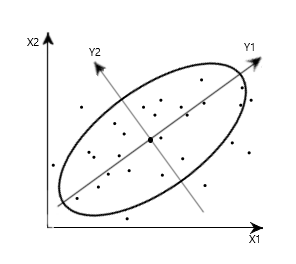
\includegraphics[scale=1]{obrazek.PNG} 
\caption{Diagram korelacyjny wyodrębnienia głównych składowych.}
\end{figure}
\bigskip
Punktem wyjścia rozważanego algorytmu jest macierz kowariancji lub macierz korelacji utworzone ze zbioru wejściowego. Zawierają one informację niezbędną do wyznaczenia głównych składowych.
\\W przypadku użycia macierzy kowariancji największy wpływ na wynik przeprowadzanego algorytmu mają zmienne o największej wariancji. Stąd też rozwiązanie to świetnie sprawdzi się w przypadku, gdy rozważane zmienne mają porównywalne wielkości: 
\begin{center}
$ A= \left[
        \begin{array}{cccc}
         \sigma_{11} & \sigma_{12} & \cdots & \sigma_{1n}\\
         \sigma_{21} & \sigma_{22} & \cdots & \sigma_{2n}\\
         \vdots & \vdots & \ddots & \vdots\\
         \sigma_{n1} & \sigma_{n2} & \cdots & \sigma_{nn}
         \end{array}
      \right]$, 
\end{center}
gdzie:
\begin{itemize}
\item $\sigma_{ii}$ - wariancja zmiennej $X_i$,
\item $\sigma_{ij}=Cov(X_i,X_j)$ - kowariancja między zmiennymi $X_i$ i $X_j$.
\end{itemize}
W przypadku, gdy zmienne różnią się znacznie w wyrażonych jednostkach, lub gdy nie są proporcjonalne zastosujemy macierz korelacji:
\begin{center}
$ B= \left[
        \begin{array}{cccc}
         1 & \rho{12} & \cdots & \rho{1n}\\
         \rho{21} & 1 & \cdots & \rho{2n}\\
         \vdots & \vdots & \ddots & \vdots\\
         \rho{n1} & \rho{n2} & \cdots & 1
         \end{array}
      \right]$, 
\end{center}
gdzie:
\begin{itemize}
\item $\rho{ij}=\frac{Cov(X_i,X_j)}{\sigma_{i}\sigma_{j}}$ - współczynnik korelacji $X_i$ i $X_j$.
\end{itemize}
\bigskip
\bigskip
Własności głównych składowych:
\begin{itemize}
\item są kombinacją liniową pierwotnych zmiennych,
\item względem siebie są ortogonalne,
\item suma wariancji pierwotnych zmiennych jest równa sumie wariancji zmiennych składowych.
\end{itemize}
\bigskip
\bigskip
Dla wspomnianej transformacji ortogonalnej, w przypadku gdy znamy wektory własne macierzy istnieje bezpośrednie równanie.
\begin{tw}
Niech $W$ będzie macierzą wektorów własnych przekształcenia $XX^T$ uporządkowaną malejąco.
Wtedy transformacja PCA jest dana wzorem $Y=W^T X$.
\end{tw}
\begin{dw}
Bez utraty ogólności załóżmy, że $X$ ma średnią zero.
\\Niech $\lambda_1\geq\lambda_2\geq...\geq\lambda_n$ będą wartościami własnymi przekształcenia $XX^T$ oraz $v_i$ odpowiadającą bazą ortogonalną. Załóżmy, że $\omega = \sum_{i=1}^n a_iv_i$ maksymalizuje wariancję oraz $w\neq v_i$.
\\Wtedy:
\begin{center}
$\omega_1 = argmax_{||\omega||=1}\omega^TXX^T\omega = argmax_{||\omega||=1}(\sum a_iv_i)^TXX^T(\sum a_iv_i)$
\\$ = argmax_{||\omega||=1}(\sum a_iv_i)^T(\sum a_i\lambda_iv_i)= argmax_{||\omega||=1}(\sum a_i)^2$.
\end{center}
Stąd $\omega_1$ maksymalizuje wariancję wtedy i tylko wtedy, gdy $\omega_1=v_1$. 
\\Znając k-1 głównych składowych k-tą znajdziemy postępując z transformacją:
\begin{center}
$X_{k-1} = X - \sum_{i=1}^{k-1}\omega_i\omega_i^TX$.
\end{center}
Podstawiając $X_{k-1}$ otrzymujemy:
\begin{center}
$\omega_k = argmax_{||x||=1}\omega^TX_{k-1}X_{k-1}^T\omega$.
\end{center}
\end{dw}
\begin{flushright}
$\Box$
\end{flushright}
Twierdzenie przedstawia użyteczną interpretację algorytmy PCA, jednakże nie jest wydajną metodą przy odnajdowaniu wektorów własnych. Poniżej zostanie przedstawiony proces odnalezienia transformacji.
\\Załóżmy, że średnia $X$ to zero. Naszym celem jest znaleźć transformację ortogonalną $W$ taką, że $WX$ jest losowym wektorem z parami niezależnych komponentów:
\begin{center}
$cov(WX) = \mathbb{E}[WX(WX)^T]
= \mathbb{E}[WX X^T W^T]
=W \mathbb{E}[XX^T]W^T
=W cov(X)W^{(-1)}$
\end{center}
Dopóki $cov(X)$ jest macierzą o wartościach dodatnich istnieje $W$, które spełnia powyższe równanie.
\\PCA jest klasyczną metodą, która pozwala odnaleźć zależności w zbiorach danych o wielu wymiarach. W wyniku tej metody otrzymujemy uporządkowaną listę cech wyznaczoną dla największych wartości wariancji przy jednocześnie najmniejszym błędzie kwadratowym (podrozdział 3.3.1). W ten sposób spośród wielu cech opisujących nasze elementy jesteśmy w stanie wybrać te najbardziej dla nas istotne w procesie rekomendacji.
\subsubsection{Rozkład Według Wartości Osobliwych (ang. Singular Value Decomposition (SVD))} 
\begin{df} \textbf{Rozkład Według Wartości Osobliwych}%https://pl.wikipedia.org/wiki/Rozk%C5%82ad_wed%C5%82ug_warto%C5%9Bci_osobliwych
%Using Linear Algebra for Intelligent Information Retrival.pdf
\\Rozkładem według wartości osobliwych $m\times n$ - wymiarowej macierzy $\mathbb{X}$, gdzie $m\geq n$ oraz $r \in \mathbb{N}$ jest rzędem macierzy $A$ nazywamy rozkład:
\begin{center}
$\mathbb{X}=\mathbb{U}\sum \mathbb{V}^T$,
\end{center}  
gdzie:
\begin{itemize}
\item $\mathbb{U}$ jest macierzą ortogonalną $m \times m$ - wymiarową,
\item $\sum $ jest macierzą diagonalną, $m \times n$ - wymiarową o nieujemnych wartościach, $\sum = diag(d_1, d_2,..., d_n)$, $n \in \mathbb{N}$ taką, że $d_i>0$ dla $1\leq i \leq r$ i $d_i=0$ dla $i\geq r+1$,
\item $\mathbb{V}$ są macierzą ortogonalną $n \times n$ - wymiarową.
\end{itemize}
\end{df}
\begin{df}\textbf{Norma Frobeniusa}%Using Linear Algebra for Intelligent Information Retrival.pdf
\\Normą Frobeniusa nazywamy:
\begin{center}
$||A||_F = \sqrt{\sum_{i=1}^m \sum_{j=1}^n |a_{ij}|^2} = \sqrt{tr A^T A}$,
\end{center}
gdzie $A$ jest macierzą $m\times n$ - wymiarową. $ A^T$ jest sprzężeniem macierzy, a $tr(A)$ śladem macierzy $A$.
\end{df}

\begin{tw}\textbf{Następstwa SVN}%Using Linear Algebra for Intelligent Information Retrival.pdf
\\Niech rozkład według wartości osobliwych macierzy $A$ będzie dany wzorem
\begin{center}
$\mathbb{X}=\mathbb{U}\sum \mathbb{V}^T$
\end{center}
gdzie $U=[u_1,u_2,...u_m]$, $V = [v_1,v_2,...v_n]$ oraz 
\\$d_1\geq d_2 \geq ... \geq d_r > d_{r+1} = ... = d_n = 0$.
\\$R(A)$ i $N(A)$ oznaczają zakres i jądro macierzy.
\\Wtedy:
\begin{enumerate}
\item właściwości rzędu macierzy: $rank(A) = r$, $N(A) = span\{v_{r+1},...,v_n \}$, $R(A) = span \{u_1,u_2,...,u_r \}$,
\item $A = \sum_{i=1}^r u_i \cdot d_i \cdot v_i^T$,
\item $||A||_F^2 = d_1^2+...+d_r^2$ i $||A||_2^2 = d_1$.
\end{enumerate}
\end{tw}

\begin{tw}\textbf{Twierdzenie Eckart - Younga}%Using Linear Algebra for Intelligent Information Retrival.pdf
\\Niech $X$ będzie macierzą $m \times n$ - wymiarową z rozkładem według wartości osobliwych $\mathbb{X}=\mathbb{U}\sum \mathbb{V}^T$, $r\in \mathbb{N} = rank(A)$ niech będzie rzędem macierzy i $r\leq p = min(m,n)$.
\\Zdefiniujmy:
\begin{center}
$A_k = \sum_{i=1}^k u_i\cdot d_i \cdot v_i^T$, 
\end{center}
wtedy
\begin{center}
$min_{rank(B) = k } ||A - B||_F^2 = ||A - A_k||_F^2 = d_{k+1}^2 + ... + d_p^2$.
\end{center}
\end{tw}
\begin{dw}
Niech $A \in \mathbb{R}^{m\times n}$ będzie macierzą o wartościach rzeczywistych, gdzie $m\geq n$.
\\Załóżmy, że
\begin{center}
$\mathbb{X}=\mathbb{U}\sum \mathbb{V}^T$
\end{center} 
jest rozkładem według wartości osobliwych macierzy $A$.
\\Chcemy pokazać, że najlepszym przybliżeniem macierzy $A$ w normie Frobeniusa (oznaczamy $||\cdot||_F$) jest
\begin{center}
$A_k = \sum_{i=1}^k u_i\cdot d_i \cdot v_i^T$,
\end{center}
gdzie $u_i$ i $v_i$ oznaczają odpowiednio $i$-te kolumny macierzy $U$ i $V$.
\\Zauważmy, że
\begin{center}
$||A - A_k||_F^2 = ||\sum_{i=k+1}^n u_i \cdot d_i \cdot v_i^T||_F^2 = \sum_{i=k+1}^n d_i^2$.
\end{center}
Stąd należy udowodnić, że $B_k = XY^T$, gdzie $X$ i $Y$ są macierzami oraz 
\begin{center}
$||A - A_k||_F^2 = \sum_{i=k+1}^n d_i^2 = ||A - B_k||_F^2$.
\end{center}
Z nierówności trójkąta, jeżeli $A = A^{`} + A^{``}$ wtedy $d_1(A)\leq d_1(A^{`}) + d_1(A^{``})$. 
\\Przez $A_k^{`}$ i $A_k^{``}$ oznaczmy przybliżenia SVD odpowiednio macierzy $A^{`}$ i $A^{``}$. 
\\Stąd dla każdego $i,j \geq 1$
\begin{center}
$d_i(A^{`}) + d_j(A^{``}) = d_1(A^{`} - A_{i-1}^{`}) + d_1(A^{``} - A_{j-1}^{``})
\geq d_1(A-A_{i-1}^{`} - A_{j-1}^{``})
\geq d_1(A-A_{i+j-2})(rank(A_{i-1}^{`} + A_{j-1}^{``}))
\geq d_{i+j-1}(A)$,
\end{center}
gdy $rank(A_{i-1}^{`} + A_{j-1}^{``}) \leq rank (A_{i+j-2})$.
\\Jeżeli 
\begin{center}
$d_{k+1}(B_k)=0$,
\end{center} 
kiedy $A^{`} = A - B_k$ i $A^{``} = B_k$ wnioskujemy, że dla $i\geq 1, j= k+1$
\begin{center}
$d_i(A-B_k)\geq d_{k+1}(A)$.
\end{center}
Stąd:
\begin{center}
$||A - B_k||_F^2 = \sum_{i=1}^n d_i(A-B_k)^2\geq \sum_{k+1}^nd_i(A)^2 = ||A-A_k||_F^2$.
\end{center}
\end{dw}
\begin{flushright}
$\Box$
\end{flushright}
\bigskip
\bigskip
Zawsze jest możliwe dokonać dekompozycji macierzy $A$ do postaci $\mathbb{X}=\mathbb{U}\sum \mathbb{V}^T$.
\\Zakładamy,że naszą macierzą wejściową jest macierz danych $A$ $m \times n$-wymiarowa odzwierciedlająca $m$ elementów oraz $n$ cech dla każdego z nich. Po przeprowadzeniu rozkładu według wartości osobliwych otrzymamy:
\begin{itemize}
\item macierz $U$ o wymiarach $m \times r$ prezentującą $m$ elementów i $r$ kategorii,
\item macierz diagonalną $\sum$ o wymiarach $r \times r$ prezentującą istotność poszczególnych kategorii,
\item macierz $V$ o wymiarach $n \times r$ prezentującą $n$ cech i $r$ kategorii.
\end{itemize}
Macierz $\sum$ zawiera pojedyncze wartości uporządkowane zawsze w porządku malejącym. Macierz $U$ jest tu interpretowana jako macierz podobieństwa elementów i kategorii, macierz $U$ natomiast jako macierz podobieństwa cech i kategorii. 
\\SVD jest powszechnie używane w celu odkrycia relacji występujących między użytkownikami i produktami.
\section{Metody eksploracji danych}
Termin eksploracja danych jest często używany jako określenie procesu odkrywania wiedzy z danych. Coraz częściej jednak terminem  "proces odkrywania wiedzy" określamy cały proces pracy z danymi, natomiast termin "eksploracja danych" odnosi się do etapu odkrywania pewnego rodzaju reguł.
\\Jak podaje w jednym ze swoich artykułów "Eksploracja danych: problemy i rozwiązania" Tadeusz Morzy metody eksploracji można podzielić na sześć klas:
\begin{itemize}
\item Odkrywanie asocjacji,
\item Klastrowanie,
\item Odkrywanie wzorców sekwencji,
\item Odkrywanie klasyfikacji,
\item Odkrywanie podobieństw w przebiegach czasowych,
\item Wykrywanie zmian i odchyleń.
\end{itemize}
W tym podrozdziale skupimy się tylko na tych, które są najczęściej stosowane w regułach rekomendujących.
\subsection{k - Najbliższych Sąsiadów}%Recomender system handbook
Algorytm k-najbliższych sąsiadów (k-NN) jest najczęściej używanym algorytmem klasyfikacji. 
Przyporządkowanie nowych elementów zostaje przeprowadzone na podstawie porównania obserwacji z $k$ najbardziej podobnymi jej obiektami ze zbioru treningowego. Podstawowa idea algorytmu mówi, że jeżeli nowy rekord znajduje się w pewnym otoczeniu, to na podstawie k - najbliższych mu obserwacji zostanie przyporządkowana do niego etykieta (klasa), której pojawienie się w rozważanym zbiorze jest najliczniejsze.
\\Niech $q$ będzie punktem dla którego chcemy odnaleźć jego klasę $l$. 
\\$X=\{\{x_1,l_1\},...,\{x_n,l_n\}\}$ niech będzie zbiorem treningowym, gdzie $x_j$ jest $j$-tym elementem zbioru, natomiast $l_j$ etykietką klasy do której zbiór należy, $j\in\{1,...,n\}$.
\\W metodzie k-NN zostaje wybrany podzbiór 
\begin{center}
$Y=\{\{y_1,l_1\},...,\{y_k,l_k\}\}$, $k\in\{1,...,n\}$
\end{center}
taki, że $Y \in X$ oraz $\sum_1^k d(q,y_k)$ jest minimalna. $Y$ zawiera więc $k$ punktów z $X$, które leżą najbliżej rozważanego punktu $q$. Następnie do punktu $q$ zostaje przyporządkowana klasa taka, że:
\begin{center}
$l=f(\{l_1,...,l_k\})$.
\end{center}
\begin{center}
\begin{figure}[H]
\centering
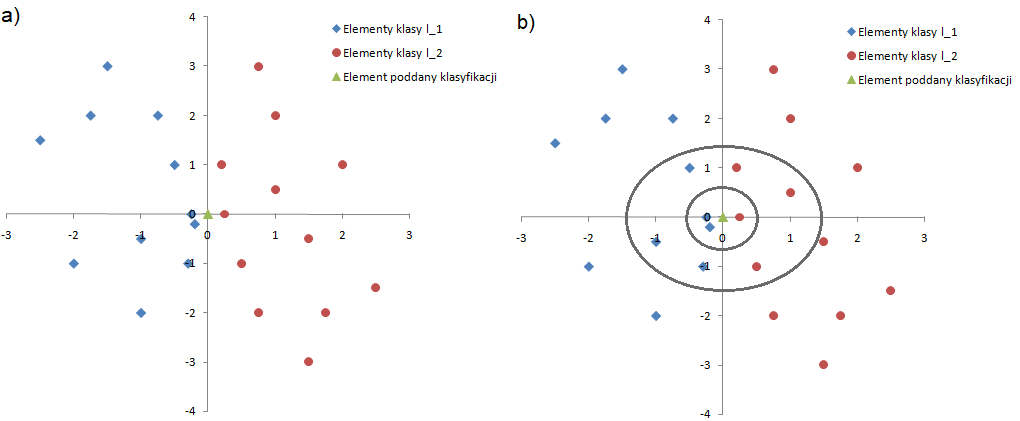
\includegraphics[scale=0.5]{kNN.PNG} 
\caption{Metoda k - Najbliższych Sąsiadów.}
\end{figure}
\end{center}
Na powyższym rysunku widzimy przykładowe zastosowanie algorytmu k-NN. W części a) przedstawiony został zbiór treningowy z podziałem na dwie klasy (rąby, koła) oraz punkt, który będziemy chcieli przyporządkować do jednej z nich (trójkąt). W części b) przedstawiono dwa koła jedno prezentuje najbliższe sąsiedztwo dla $k = 3$, drugie dla $k = 9$. W obu przypadkach nowy punkt (trójkąt) zostanie przyporządkowany do klasy $l_1$. Warto również zauważyć, że znajduje się on na granicy dwóch klastrów.
\\
\\Jak wyżej opisana metoda przyporządkowuje wybranemu rekordowi najbardziej mu podobne w przypadku, gdy dane są więcej niż dwuwymiarowe?
\\Wykorzystywane są tutaj wcześniej opisane miary odległości z których najczęściej stosowaną jest odległość euklidesowa.
\\
\\Najtrudniejszym zadaniem przy przeprowadzaniu algorytmu k-NN jest wybór $k$. Jeżeli $k$ będzie zbyt małe - klasyfikator stanie się bardzo wrażliwy, jeżeli jednak $k$ będzie zbyt duże sąsiedztwo może zawierać zbyt dużo punktów z innych klas. Rozważając przypadek z Rysunku 3.2 łatwo zauważyć, że nawet mała zmiana w obserwacjach zbioru treningowego może doprowadzić do zmiany wyniku.

\subsection{k-Średnich}%Analiza skupień Agnieszka Nowak-Brzezińska
Algorytm k-średnich jest prostym i zarazem efektywnym algorytmem grupowania.
\\Głównym celem algorytmu jest podział pewnego zbioru $X$:
\begin{center}
$X = \{x_i = (x_{i1},...,x_{id}) : i \in \{1,...,N\}\}$,
\end{center}
gdzie $x_i$ jest $d$-wymiarowym wektorem cech opisującym obiekt na podzbiory.
\\W wyniku grupowania $n$ - elementowego zbioru $X$ na $k$ podgrup jest macierz podziału $A$ o wymiarach $k\times n$ . Każdy z elementów tej macierzy $a_{ik}$ oznacza stopień w jakim wektor $x_k$ przynależy do grupy.
\\Na wstępie algorytmu ustalamy wartość parametru $k$ jako liczbę grup, które zostaną wyodrębnione. Wybieramy $k$ reprezentantów, które stanowią prototypy grup.
\begin{center}
\begin{figure}[H]
\centering
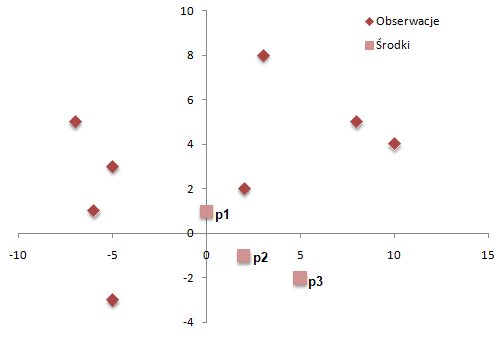
\includegraphics[scale=0.8]{ks_0.PNG} 
\caption{Metoda k-średnich. Wybór początkowych środków.}
\end{figure}
\end{center}
W powyższym przykładzie (Rysunek 3.3) wybranymi środkami są punkty p1, p2, p3.
\\
Kolejnym krokiem jest przypisanie każdego z elementów do najbliższej mu grupy.
\begin{center}
\begin{figure}[H]
\centering
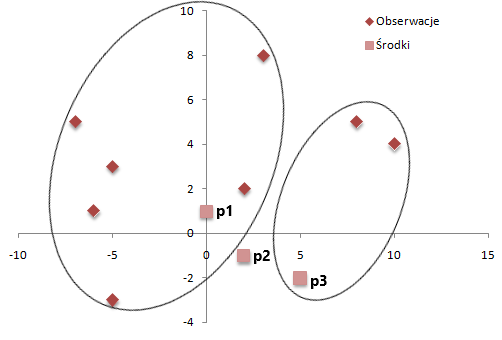
\includegraphics[scale=0.8]{ks_1.png} 
\caption{Metoda k-średnich. Przypisanie elementów do grup.}
\end{figure}
\end{center}
Dla każdej z tak ustalonych grup obliczamy średnią arytmetyczną współrzędnych, które staną się kolejnymi środkami.
\begin{center}
\begin{figure}[H]
\centering
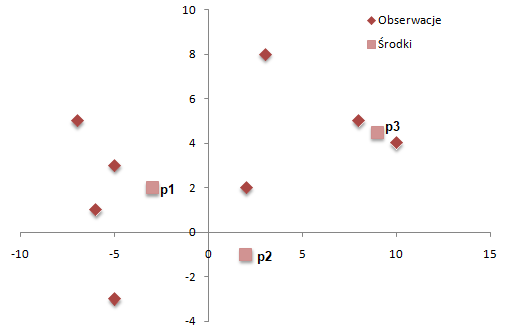
\includegraphics[scale=0.8]{ks_2.png} 
\caption{Metoda k-średnich. Wybór nowych środków.}
\end{figure}
\end{center}
Kroki te są wykonywane do momentu występowania migracji między obiektami.
\\W algorytmie k-średnich liczba grup pozostaje więc niezmienną, zmienna jest tylko przynależność do grup.
\\W metodzie tej poszukiwanie optymalnego podziału odpowiada wyznaczaniu takich grup, które minimalizują następującą funkcje:
\begin{center}
$J(u,A) = \sum_{i=1}^k \sum_{k=1}^N b_{ki}d^2(u_i,x_k)$,
\end{center}
gdzie 
\begin{itemize}
\item $d(u,x)$ oznacza odległość elementu $x$ od grupy wyznaczonej przez środek $u$,
\item $N$ to liczebność zbioru $X$,
\item $A$ oznacza macierz podziału.
\end{itemize}
 
\subsection{drzewa decyzyjne-?}
\subsection{regresja wielowymiarowa - logistyczna - ?}
\subsection{Sztuczna Sieć Neuronowa}
Sztuczna Sieć Neuronowa jest klasyfikatorem opartym na systemie działania ludzkiego mózgu. Składa się z neuronów, które są połączone ze sobą synapsami. Te proste elementy połączone są w sieć, która posiada możliwość uczenia się problemów klasyfikacyjnych.
\\
\subsection{Maszyna Wektorów Nośnych}
Maszyny Wektorów Nośnych (ang. Support Vector Machines (SVM)) jest algorytmem uczenia maszynowego używanym zarówno w przypadku zadań klasyfikacji jak i regresji. Głównym celem algorytmu jest znalezienie w przestrzenie $n$ - wymiarowej hiperpłaszczyzny, która wyraźnie sklasyfikuje obserwacje i podzieli na dwie klasy maksymalizując odległość między obserwacjami. Podejście to pozwala uniknąć błędnego przyporządkowania marginalnych obserwacji w przyszłości.
\begin{center}
\begin{figure}[H]
\centering
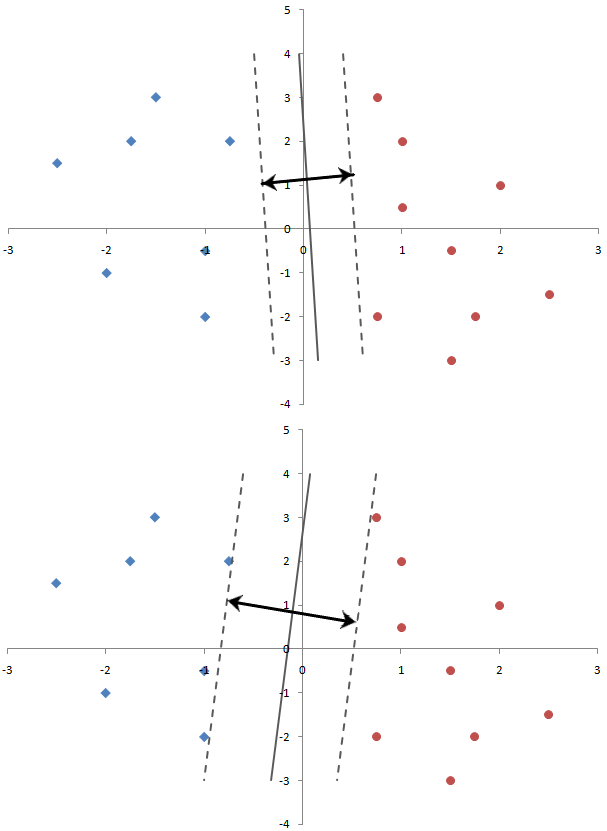
\includegraphics[scale=0.5]{SVM.PNG} 
\caption{Maszyna Wektorów Nośnych - maksymalizacja odległości między klasami.}
\end{figure}
\end{center}
Aby formalnie zdefiniować Maszyna Wektorów Nośnych zacznijmy od zdefiniowania problemu klasyfikacji.
\begin{df}\textbf{Klasyfikacja}
\\Nich w przestrzeni $\Omega$ znajdują się wektory danych $x_i \in \mathbb{R}^n$, $i\in \{1,...,n\}$. $P$ niech będzie próbą uczącą.
\\Wtedy:
\begin{center}
$P = \{(x_i,c_i): x_i \in \mathbb{R}^n, c_i \in \{1,-1\}\}_{i=1}^N$.
\end{center}
\end{df}
\bigskip
Należy znaleźć klasyfikator dzielący całą przestrzeń $\Omega$ na dwie klasy $\{-1,1\}$, który pozwoli na przyporządkowywać nowego elementu do klasy. Szukamy funkcji $f(x)$ - granicy między klasami.

\begin{df}\textbf{Liniowa Separowalność}%https://towardsdatascience.com/support-vector-machine-introduction-to-machine-learning-algorithms-934a444fca47
\\Dwie klasy nazywamy liniowo separowalnymi, jeżeli istnieje hiperpłaszczyzna $f(x)$ postaci:
\begin{center}
$f(x) = w^T x +b$
\end{center}
taka, że:
\begin{center}
$\left\{\begin{array}{ll}
f(x_i)>0, &    x_i\in\{1\}\\
f(x_i)<0, &    x_i\in\{-1\}.
\end{array} \right.$
\end{center}
\end{df}
\bigskip
\bigskip
\bigskip
Liniową separowalność definiujemy więc za pomocą funkcji:
\begin{center}
$\langle w,x \rangle + b = 0$, 
\end{center}
gdzie $w, b$ są parametrami spełniającymi założenia modelu:
\begin{center}
$f(x) = 
\left\{\begin{array}{lll}
1, & gdy &   \langle w,x \rangle + b > 0\\
-1, &   gdy &   \langle w,x \rangle + b < 0.
\end{array} \right.$
\end{center}
Parametry $w$ i $b$ wyznaczamy w taki sposób, by odległość między płaszczyznami
\begin{center}
$ b_{i1}$ $\langle w,x \rangle + b = 1$,
\\$ b_{i2}$ $\langle w,x \rangle + b = -1$
\end{center}
była maksymalna.
\\Zatem
\begin{center}
$f(x) = 
\left\{\begin{array}{lll}
1, & gdy &   \langle w,x \rangle + b \geq 1\\
-1, &   gdy &   \langle w,x \rangle + b \leq -1,
\end{array} \right.$
\end{center}
oraz szukana odległość wyznaczana jest przez maksymalizowanie funkcji 
\begin{center}
Margin (odległość)=$\frac{2}{||w||^2}$.
\end{center}
Jest to fakt równoważny minimalizowaniu funkcji odwrotnej do powyższej
\begin{center}
$L(W) = \frac{||w||^2}{2}$,
\end{center}
przy ograniczeniach
\begin{center}
$y_i(\langle w,x \rangle + b) \geq 1$.
\end{center}
Problem ten nazywamy problemem optymalizacji kwadratowej i rozważamy przy użyciu mnożników Lagrange'a. Minimalizujemy więc funkcję Lagrange'a:
\begin{center}
$L(w,b,\alpha)=\frac{1}{2}||w||^2 - \sum_{i=1}^n \alpha_i(y_i(\langle w,x \rangle + b)-1)$, 
\end{center}
gdzie
$\alpha_i \geq 0$ dla $i \in \{1,...,n\}$ to mnożniki Lagrange'a spełniające ograniczenia Karusha-Kuhna-Tuckera:
\begin{itemize}
\item $\alpha_i \geq 0$,
\item $\alpha_i(y_i(\langle w,x \rangle + b)-1) = 0$.
\end{itemize}
Możemy zauważyć, że w konsekwencji mnożniki Lagrange'a są niezerowe tylko dla wektorów nośnych. Liczba parametrów do oszacowania pozostaje jednak nadal zbyt duża. Częstym podejściem w tym przypadku jest przejście na postać dualną zadania optymalizacyjnego.
Maksymalizujemy tu funkcję:\begin{center}
$\sum_{i=1}^n \alpha_i - \frac{1}{2} \sum_{i=1}^n \sum_{j=1}^{n} \alpha_i \alpha_j y_i y_j(x_i \times x_j)$,
\end{center}
przy ograniczeniach:
\begin{itemize}
\item $\alpha_i \geq 0$,
\item $\forall_i \sum_{i=1}^n \alpha_i y_i =0$.
\end{itemize}
\bigskip
\bigskip
\bigskip
Jeżeli elementy nie są jednak separowalne liniowo:
\begin{center}
\begin{figure}[H]
\centering
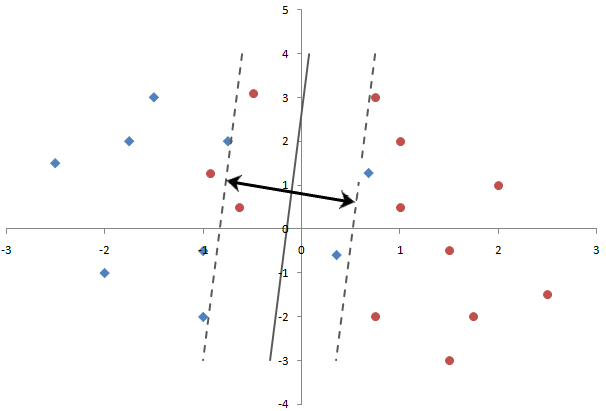
\includegraphics[scale=0.5]{SVM2.PNG} 
\caption{Maszyna Wektorów Nośnych - elementy nieseparowalne liniowo.}
\end{figure}
\end{center}
wprowadzamy klasyfikator \textbf{Soft Margin SVM} oraz zmienne osłabiające (pomocnicze).
\\W tym przypadku należy poddać minimalizacji funkcję:
\begin{center}
$L(w) = \frac{||w||^2}{2} + C \sum_{i=1}^n \varepsilon$,
\end{center}
gdzie parametr $C$ ocenia starty związane z każdym błędnie zaklasyfikowanym punktem.
\\Funkcja $f(x)$ jest natomiast dana wzorem:
\begin{center}
$f(x) = 
\left\{\begin{array}{lll}
1, & gdy &   \langle w,x \rangle + b \geq 1 - \varepsilon\\
-1, &   gdy &   \langle w,x \rangle + b \leq -1 + \varepsilon.
\end{array} \right.$
\end{center}
Interpretacja rozwiązań:
\begin{itemize}
\item $\varepsilon_n =0$ i $\alpha_i =0$ - poprawne zaklasyfikowanie obserwacji, obserwacja leży poza marginesem,
\item $\varepsilon_n =0$ i $0<\alpha_i <C$ - poprawne zaklasyfikowanie obserwacji, obserwacja leży na jednej z płaszczyzn ograniczających margines,
\item $0<\varepsilon_n <1$ i $\alpha_i =C$ - poprawne zaklasyfikowanie obserwacji, obserwacja leży wewnątrz marginesu,
\item $\varepsilon_n \geq 1$ i $\alpha_i =C$ - niepoprawne zaklasyfikowanie obserwacji.
\end{itemize}

\section{Szacowanie Błędów Obliczeń}
\subsection{Ocena Dokładności Metody}%RecommenderSystemsHandbook
Kolejna kwestia często poruszana w regułach rekomendujących to dokładność przewidywań. Jak oceniamy, czy uzyskany przez nas wynik jest wystarczająco dokładny? 
\\Załóżmy, że dla użytkownika $u$ i elementu $i$ ze zbioru testowego $P$ dostarczamy predykcję $\widehat{r_{(u,i)}}$. Aby ocenić jakość wyniku należy porównać ją ze znaną wartością $r_{(u,i)}$.
\\
\\Najczęściej używanymi miarami dokładności modelu są:
\begin{itemize}
\item \textbf{Średni Błąd (Mean Error)}
\begin{center}
$ME = \frac{1}{|P|}\sum_{(u,i)\in P}(\widehat{r_{(u,i)}}-r_{(u,i)})$   
\end{center}

\item \textbf{Średni Błąd Bezwzględny (Mean Absolute Error)}
\begin{center}
$MAD = \frac{1}{|P|}\sum_{(u,i)\in P}|\widehat{r_{(u,i)}}-r_{(u,i)}|$   
\end{center}

\item \textbf{Średni Błąd Kwadratowy (Mean Squared Error)}
\begin{center}
$MSE = \frac{1}{|P|}\sum_{(u,i)\in P}(\widehat{r_{(u,i)}}-r_{(u,i)})^2$   
\end{center}
\end{itemize}
Funkcja kwadratowa jest funkcją monotoniczną co pozwala na dość częste zastępowanie średniego błędu kwadratowego przez średnią kwadratową błędów \textbf{(Root Mean Squared Error (RMSE))}.
\begin{center}
$RMSE = \sqrt{MSE}$
\end{center} 
\textbf{Normalized RMSE (NRMSE)} oraz \textbf{Normalized MAE (NMAE)} są znormalizownymi, przez użycie zakresu wartości $r_{max} - r_{min}$, wersjami błędów RMSE i MAE.
\\Kolejnym rodzajem powszechnie używanego błędu jest \textbf{Average RMSE}, który pozwala na użycie sum ważonych. Niech $w_i>0$ będzie wagę dla elementu $i$ i $\sum w_i = 1$. 
\begin{center}
$ARMSE = \sqrt{\sum_{(u,i)\in P}w_{i}(\widehat{r_{(u,i)}}-r_{(u,i)})^2}$ 
\end{center}

\subsection{Ocena Precyzji Użyteczności}
W regułach rekomendujących częstymi są przypadki, gdzie systemy nie będą przewidywać konkretnych preferencji użytkownika, jak oceny ale samo prawdopodobieństwo podjęcia przez użytkownika akcji.
\\Oceniając taki model wybieramy przykładowego użytkownika i ukrywamy kilka wybranych przez niego elementów aby spróbować przewidzieć zestaw elementów jakie użytkownik będzie chciał wybrać. W poniższej tabeli zostały zaprezentowane rezultaty jakie są możliwe do otrzymania przy przeprowadzaniu takiego testu:
\begin{center}
\begin{tabular}{|r|r|r|} \hline
 & Zarekomendowane & Niezarekomendowane  \\
\hline 
Wybrane & prawda-pozytywnie & fałsz-negatywnie \\
przez użytkownika &(pp)&(fn) \\
\hline
Niewybrane & fałsz-pozytywnie & prawda-negatywnie \\
przez użytkownika &(fp)&(pn) \\
\hline
\end{tabular}
\end{center}
Zakładamy, że elementy nieużyte przez użytkownika nie zostałyby użyte również w przypadku gdy zostałyby zarekomendowane. Założenie to może okazać się jednak błędne, ponieważ w wyniku rekomendacji możemy otrzymać interesujące propozycje, których użytkownik nie brał pod uwagę. Jest to powód dlaczego wynik $fp$ jest bardzo często przeszacowany.
\\W celu porównania algorytmów możemy posłużyć się następującymi statystykami:
\begin{center}
Precyzja (ang. Precision) $= \frac{|pp|}{|pp|+|fp|}$, %czy liczność w tym przypadku może zostać zapisana przez | | 
\\\textit{Wskaźnik pp (ang. Recall / True Positive Rate)} $ = \frac{|pp|}{|pp|+|fn|}$,
\\\textit{Wskaźnik fp (ang. False Positive Rate)} $ = \frac{|fp|}{|fp|+|pn|}$.
\end{center}
Często jednak jest tu obserwowana zależność, która pokazuje, że przy wydłużaniu się listy rekomendacji rośnie wartość \textit{wskaźnika pp} i jednocześnie maleje \textit{precyzja}. Dla stałej długości listy rekomendacji porównanie precyzji algorytmów jest jak najbardziej miarodajne. Niemniej jednak porównanie precyzji, gdzie długości list rekomendacji są różne jest często bardzo trudne. Zostaje zatem wyznaczona krzywa przedstawiająca kompromis między \textit{wskaźnikiem pp} i \textit{precyzją}, lub między \textit{wskaźnikiem pp} i \textit{wskaźnikiem fp}. Formalnie pierwsza krzywa jest nazywana \textbf{krzywą precyzji (ang. precision - recall curve)} natomiast druga \textbf{krzywą ROC (ang. Receiver Operating Characteristic)}.

\subsection{Ocena Rankingów}
W poprzedniej sekcji została omówiona metoda wyboru odpowiedniego modelu rekomendującego. Każdy z takich modeli kończy się przedstawieniem pewnej listy rekomendowanych elementów. Często jednak również kolejność elementów jest bardzo ważna i ma duży wpływ na wybory użytkowników.
\\W tej części zostaną zaprezentowane metody służące do oceny otrzymanych na podstawie modelu rankingów i pomagające zapewnić odpowiedni porządek rekomendowanych elementów. Jeżeli elementy posiadają oceny (np. użytkowników) intuicyjnym jest stworzyć ranking przez uporządkowanie tych ocen w malejący sposób. W przypadku gdy jednak nie mamy takich danych lub nie jest odpowiednie tworzenie takiego rankingu użyjemy \textbf{znormalizowanej miary opartej na odległości (ang. Normalized Distance-based Performance Measure (NDPM): }
\\
\\Niech $r_{ui}$ będzie rankingiem odniesienia i $\widehat{r}_{ui}$ rankingiem stworzonym przez wybrany system rekomendującym $n_u$ elementów $i$ użytkownikowi $u$. 
\\Ponadto niech:
\begin{center}
$C^{+} = \sum_{i<j} sgn(r_{ui} - r_{uj})sgn(\widehat{r}_{ui}-\widehat{r}_{uj})$
\\$C^{-} = \sum_{i<j} sgn^{2}(r_{ui} - r_{uj})sgn(\widehat{r}_{uj}-\widehat{r}_{ui})$
\\$C^{u} = \sum_{i<j} sgn^{2}(r_{ui} - r_{uj})$
\\$C^{s} = \sum_{i<j} sgn(\widehat{r}_{ui}-\widehat{r}_{uj})$
\\$C^{0}=C^{u}-(C^{+}-C^{-})$, gdzie
\end{center}
$C^{u}$ jest liczbą par dla których ranking referencyjny okazuje się lepszą możliwością, 
\\$C^{+}$ i $C^{-}$ to liczba par z poprawną i niepoprawną kolejnością,
\\$C^{0}$ jest liczbą par dla których ranking referencyjny nie jest wiążący, kiedy ranking systemu rekomendującego jest.
\\
\\Ostatecznie NDPM definiujemy w następujący sposób:
\begin{center}
$NDPM = \frac{C^{-} + 0.5 C^{0}}{C^{u}}$
\end{center}
Powiązania w rankingu referencyjnym pojawiają się naturalnie, kiedy znamy preferencje użytkownika (np. przydziela on oceny). Czasami jednak rankingi są bardziej specyficzne (np. kiedy dajemy użytkownikowi wybór między dwoma elementami). Wtedy też system rekomendujący nie powinien tworzyć rankingu klasyfikując jedne elementy wyżej niż inne. W takich przypadkach przychodzą nam z pomocą 
\\\textbf{miara Kendall's $\tau$}:
\begin{center}
$\tau = \frac{C^{+} - C^{-} }{\sqrt{C^{u}}\sqrt{C^{s}}}$
\end{center}
oraz \textbf{miara Spearman's $\rho$}:
\begin{center}
$\rho = \frac{1}{n_{u}}\frac{\sum_i (r_{iu} - \overline{r})(\widehat{r}_{iu}-\overline{\widehat{r}})}{\sigma(r)\sigma(\widehat{r})}$,
\end{center}
gdzie $\overline{r}$ i $\overline{\widehat{r}}$ oznaczają średnie, natomiast $\sigma(r)$ i $\sigma(\widehat{r})$ odchylenia standardowe.




\chapter{Modele tworzenia rekomendacji}
Systemy rekomendujące mogą zostać podzielone na systemy oparte na kontekście i systemy oparte na użytkownikach. W pierwszym przypadku eksploracja danych jest dokonywana pod względem zawartych w treści rozważanego elementu cech. Główne założenie mówi, że jeżeli użytkownik wybrał przedmiot A w przeszłości oraz przedmiot B jest podobna do A, to użytkownik będzie skłonny wybrać również przedmiot B. W systemach opartych na użytkownikach badaniu podlegają natomiast zależności, które występują między produktami, a użytkownikami. Idea rozważana pod tym hasłem mówi, że jeżeli użytkownicy A i B wykazują podobieństwo oraz użytkownik A zaopiniuje pewien przedmiot, którego użytkownik B jeszcze nie ocenił, to prawdopodobnie opinia użytkownika B będzie podobna do opinii użytkownika A.


\section{Systemy rekomendujące oparte na treści (Content-based recommender systems):}
\subsection{Problem}
Rozważmy sytuację w której szukamy przyjemnej lektury na zimowy wieczór. Zaczynamy od przeglądania tytułów wśród interesujących nas gatunków. Następnie spojrzymy zapewne na oceny jakie inni czytelnicy wydali na temat danej pozycji. Analizując wartość uzyskanych ocen ostatecznie podejmujemy na ich podstawie najbardziej odpowiednią dla nas decyzję. 

\subsection{Algorytm}
Metody rozwiązywania podobnych problemów często spotykane są w matematyce. Jednym z przykładów są systemy oparte na treści, które wyróżnia ukierunkowanie na spersonalizowany poziom użytkownika oraz treści produktu. Głównym celem tej metody jest scharakteryzowanie cech, które użytkownik ceni, a następnie zasugerowanie mu produktów, które te cechy posiadają. Wspomniana metoda opiera się na obliczaniu podobieństw oraz wykorzystuje zadania uczenia maszynowego, takie jak klasyfikacja.
\\
\\
W typie rekomendacji opartym na treści stworzenie rekomendacji i wygenerowanie listy elementów, które mogę być odpowiednie użytkownikowi możemy przedstawić w trzech krokach:
\begin{enumerate}
\item{Wygenerowanie profilu produktu}
\item{Wygenerowanie profilu użytkownika}
\item{Rozpoznanie cech produktu odpowiednich dla użytkownika}
\end{enumerate}


\subsection{Wygenerowanie profilu produktu}
W większość systemów rekomendacji opartych na treści można zauważyć użycie prostych modeli wyszukujących. Jednym z najbardziej popularnych jest Model Przestrzeni Wektorowej (\textit{ang. Vector Space Model}) z algorytmem TF-IDF (\textit{ang. TF – term frequency, IDF - inverse document frequency}). Jest to przestrzenna forma reprezentacji dokumentów, gdzie dokument $i$ jest reprezentowany przez wektor w przestrzeni n-wymiarowej $x_{i}$, a każdy z $n$ wymiarów stanowi rozważaną cechę produktu. Dla danych w formie dokumentów tekstowych cechami, które pomagają scharakteryzować temat dokumentu, np. artykułu na stronie internetowej są słowa. Dla każdego ze słów zostaje obliczona wartość funkcji TFIDF (została ona dokładnie omówiona poniżej). W końcowym etapie słowa, które otrzymały najwyższe wyniki zostają uznane za charakteryzujące rozważany dokument.
\\
\\Formalnie rzecz ujmując każdy z dokumentów jest przedstawiony za pomocą wektora wag, gdzie waga w odpowiedni sposób wyraża zależność między dokumentem, a badanym terminem.
\\
\\Niech \begin{math} P = \{p_1, p_2,...,p_n\}, n\in{\mathbf{N}} \end{math} będzie zestawem dokumentów / analizowanych przedmiotów. Natomiast \begin{math}C = \{c_1, c_2,...,c_n\}, n\in{\mathbf{N}} \end{math} zestawem cech rozważanych w przedmiotach. Każdy z dokumentów \begin{math} p_j, j\in{\{1,...,n\}} \end{math} jest reprezentowany jako wektor w przestrzeni wektorowej n-wymiarowej. Zatem \begin{math} p_j = [w_{1j}, w_{2j},...,w_{nj}] \end{math}, gdzie \begin{math} w_{kj} \end{math}  jest wagą dla cechy \begin{math} c_k \end{math} w dokumencie  \begin{math} p_j \end{math}.
\\
\\
Do generowania profilu produktu używany jest wspomniany wcześniej algorytm TFIDF pozwalający policzyć względną ważność powiązania cechy z przedmiotem. Zakładamy tu, że:
\begin{itemize}
\item rzadkie cechy są równie istotne jak częste (założenie IDF),
\item kilkukrotne wystąpienie terminu w rozważanym dokumencie jest równie istotne jak pojedyncze (założenie TF),
\item długość dokumentu (filmu, książki) nie ma znaczenia (założenie normalizacji).  
\end{itemize}
Możemy więc powiedzieć, że jeżeli termin występuje często w konkretnym przedmiocie rozważań (TF) i równocześnie rzadko w pozostałych elementach zboru (IDF) ma większe prawdopodobieństwo stać się jedną z istotnych cech rozważanych w temacie. Ponadto normalizacja wektorów wag pozwala zrównoważyć wartość wyników i umożliwia ich porównywanie w dalszej analizie.
\\
\\Powyższe założenia odzwierciedla funkcja TFIDF:
\begin{center}
\begin{math}
TFIDF(t_k, d_j) = TF(c_k, p_j) * IDF,
\end{math}
\end{center}
gdzie:
\begin{itemize}
\item \begin{math}TF(c_k, p_j)  \end{math} (macierz \textit{term frequency}) przedstawia odniesienie każdego z podanych terminów do każdego z badanych elementów:
\begin{center}
\begin{math}
TF(c_k, p_j)=\frac{f_{k,j}}{\max_{z}f_{z,j}},
\end{math}
\end{center}
$\max_{z}f_{z,j}$ - maksymalna w odniesieniu do wszystkich cech $c_z$, które pojawiły się w dokumencie $p_j$ częstotliwość wystąpień ($f_{z,j}$) 

\item \begin{math}IDF \end{math} (\textit{inverse dokument frequency}) wyraża się formułą:
\begin{center}
\begin{math}IDF = \log \frac{N}{n_k} \end{math}
\end{center}
$N$ - całkowita liczba dokumentów w zbiorze,
\\$n_k$ - liczba dokumentów w których cecha $c_k$ wystąpiła przynajmniej raz.
\end{itemize}
Ponadto w związku z założeniem o normalizacji wagi, które zostały uzyskane w wyniku \begin{math}
TFIDF(t_k, d_j)
\end{math} poddane zostaną metodzie transformacji kosinusowej: 
\begin{center}
\begin{math}
w_{k,j} = \frac{TFIDF(t_k, d_j)}{\sqrt{\sum_{i=1}^{|T|}{TFIDF(t_i, d_j)}^2}}.
\end{math}
\end{center}
Tak wygenerowany został zbiór słów, które są reprezentacją danego dokumentu oraz jego tematu. Ostatnim krokiem przed zarekomendowaniem pozycji czytelnikom jest wyestymowanie podobieństw występujących między poszczególnymi dokumentami. Naturalnymi miarami odległości, które można tu wykorzystać są:
\begin{itemize}
\item współczynnik Jaccarda mierzący odległość między zbiorami słów,
\item podobieństwa kosinusów mierzące odległość między wektorami:

\begin{center}
\begin{math}
sim(p_i,p_j) = \frac{\sum_{i=k} w_{k,i}\cdot w_{k,j}}{\sqrt{\sum_{k=1}{w_{k,i}}^2} \cdot \sqrt{\sum_{k=1}{w_{k,j}}^2}}.
\end{math}
\end{center}
Przy estymowaniu odległości kosinusów między dwoma dokumentami elementami wektora są słowa, które zostały wybrane na podstawie wcześniej przeprowadzonego algorytmu. W wektorze tym wartość $1$ oznacza, że słowo pojawiło się w zbiorze opisującym dokument, natomiast $0$ oznacza sytuację przeciwną.
\end{itemize}

\subsection{Wygenerowanie profilu użytkownika}
Przy generowaniu wektora opisującego rozważane dokumenty należy uwzględnić komponenty opisujące preferencje użytkowników. Dla każdego użytkownika $u$ przedstawiamy jego preferencje w postaci wektora $x_u$, gdzie użytkownik pozycjonuje element $i$ poprzez wektor cech $x_i$.
\subsection{Rozpoznanie cech produktu odpowiednich dla użytkownika} 
Proces rekomendacji bazuje na dopasowaniu cech profilu użytkownika i wartości opisujących treść obiektu. Rezultatem jest stwierdzenie czy rozważany kandydat jest zainteresowany analizowanym przedmiotem. Zainteresowanie użytkownika danym przedmiotem można wyestymować używając podobieństwa cosinusów. Rozważmy dokument, gdzie użytkownik wyraża zainteresowanie większością cech w wektorze $x_i$ opisującym dokument $i$. Otrzymamy cosinus kąta między użytkownikiem i dokumentem będący dodatnim ułamkiem. Oznacza to, że kąt będzie bliski $0^{o}$ a tym samym odległość między wektorami będzie mała. W przypadku przeciwnym otrzymamy cosinus bliski zeru lub mniejszy od zera, oznacza to kąt należący do przedziału $(90^{o};180^{o})$ oraz małe podobieństwo między rozważanymi wektorami.

\subsection{Przykład}
Aby dokładnie przyjrzeć się metodom opartym na treści rozważmy wcześniej przytoczony problem oparty na książkach.
Poniższa tabela przedstawia tytuły kilku randomowo wybranych książek wraz z gatunkami.
\begin{center}
\begin{tabular}{|r|r|} \hline
\textbf{Książka} & \textbf{Gatunek} \\
\hline 
Władza Absolutna & Kryminał  \\
\hline 
Patrioci & Proza współczesna \\
\hline 
Proxima & Powieść fantastycznonaukowa \\
\hline 
Strażacy & Literatura faktu \\
\hline 
Gra o Śmierć & Romans \\
\hline 
Cyrk & Komedia \\
\hline
\end{tabular}
\end{center}
Przez wykorzystanie algorytmu TFIDF stworzymy profil każdej z książek.
Pierwszym etapem algorytmu jest stworzenie macierzy „term frequency”. W tym przypadku jej wypełnienie przedstawia odniesienie każdego z podanych terminów do każdej z książek. Załóżmy, że 1 oznacza iż książka reprezentuje cechy danego gatunku, natomiast 0 oznacza brak takich cech. 
\\
\\
\footnotesize{
\begin{tabular}{|r|r|r|r|r|r|r|r|r|} \hline
Książka  & Kry- & Proza &  Powieść & Litera- & Romans & Komedia & Książka & Thriller\\
/ & minał & współ- &  fantastycz- & tura &  &  & akcji & \\
Gatunek & & czesna &  nonaukowa & faktu &  &  &  & \\
\hline \hline 
Władza & &  &  &  &  & &  &  \\
Absolutna & 1 & 0 & 0 & 0 & 0 & 0 & 1 & 0 \\
Patrioci & 0 & 1 & 0 & 0 & 0 & 0 & 1 & 0 \\
Proxima & 0 & 1 & 1 & 0 & 0 & 0 & 0 & 0 \\
Strażacy & 0 & 0 & 0 & 1 & 0 & 0 & 1 & 0 \\
Gra & &  &  &  &  & &  &  \\
o Śmierć & 0 & 0 & 0 & 0 & 1 & 0 & 0 & 1 \\
Cyrk & 1 & 0 & 0 & 0 & 0 & 1 & 0 & 0\\
\hline
\end{tabular}
}
\normalsize{
\\
\\Zbadajmy teraz "inverse dokument frequency".
\begin{center}
\begin{math}IDF = \log \frac{N}{n_k} \end{math}
\end{center}
W rozważanym przypadku $N$ to liczba książek, natomiast $n_k$ to całkowita liczba wystąpień "term frequency", uzyskana dla wszystkich dokumentów.
}
\begin{center}
\begin{tabular}{|r|r|r|r|r|r|r|r|} \hline
Kry- & Proza &  Powieść & Litera- & Romans & Komedia & Książka & Thriller\\
minał & współ- &  fantastycz- & tura &  &  & akcji & \\
 & czesna &  nonaukowa & faktu &  &  &  & \\
\hline \hline 
1.098612 & 1.098612 & 1.791759 & 1.791759 & 1.791759 & 1.791759 & 0.693147 & 1.791759 \\
\hline
\end{tabular}
\end{center}
\normalsize{Mając stworzona macierz "term frequency" oraz wektor "inverse dokument frequency" przejdźmy do ostatniego kroku i stwórzmy macierz TFIDF dla rozważanego przypadku:}
\begin{center}

\footnotesize{
\begin{tabular}{|r|r|r|r|r|r|r|r|r|} \hline
Książka  & Kry- & Proza &  Powieść & Litera- & Romans & Komedia & Książka & Thriller\\
/ & minał & współ- &  fantastycz- & tura &  &  & akcji & \\
Gatunek & & czesna &  nonaukowa & faktu &  &  &  & \\
\hline 
Władza & &  &  &  &  & &  &  \\
Absolutna & 1.098612 & 0 & 0 & 0 & 0 & 0 & 0.693147 & 0 \\
\hline
Patrioci & 0 & 1.098612 & 0 & 0 & 0 & 0 & 0.693147 & 0 \\
\hline
Proxima & 0 & 1.098612 & 1.791759 & 0 & 0 & 0 & 0 & 0 \\
\hline
Strażacy & 0 & 0 & 0 &1.791759 & 0 & 0 & 0.693147 & 0 \\
\hline
Gra & &  &  &  &  & &  &  \\
o Śmierć & 0 & 0 & 0 & 0 & 1.791759 & 0 & 0 & 1.791759 \\
\hline
Cyrk & 1.098612 & 0 & 0 & 0 & 0 & 1.791759 & 0 & 0\\
\hline
\end{tabular}
}
\end{center}
\normalsize{
Zakończyliśmy generowanie profilu przedmiotu, przejdźmy więc do wygenerowania profilu użytkownika. 
\\Rozważmy zbiór danych, który przedstawia informacje o czytelnikach i książkach. W poniższym zestawieniu 1 oznacza, że dana osoba przeczytała książkę, natomiast puste miejsce, że nie podjęła się lektury.
\begin{center}
\begin{tabular}{|r|r|r|r|r|r|r|} \hline
Książka/Czytelnik & Anna & Maciej & Bartek & Ewa & Sandra & Kacper \\
\hline \hline 
Władza Absolutna & 1 & 1 & & 1 & 1 &  \\
Patrioci &  & 1 & 1 & 1 & 1 &  \\
Proxima & 1 & 1 & 1 & 1 & 1 & 1 \\
Strażacy & 1 & 1 & 1 & 1 & 1 & 1 \\
Gra o Śmierć & 1 & 1 & 1 & 1 & 1 &  \\
Cyrk & 1 & 1 & 1 & 1 & 1 & 1 \\
\hline
\end{tabular}
\end{center}
Profil użytkownika powinien zawierać jego preferencje dotyczące cech danego przedmiotu, w tym przypadku będą to preferencje dotyczące gatunku książki. Iloczyn skalarny zbudowany na TFIDF i macierzy preferencji użytkowników przedstawi powinowactwo każdego z użytkowników do każdego z rozważanych gatunków książki. 
\begin{center}
\footnotesize{
\begin{tabular}{|r|r|r|r|r|r|r|r|r|} \hline
Książka  & Kry- & Proza &  Powieść & Litera- & Romans & Komedia & Książka & Thriller\\
/ & minał & współ- &  fantastycz- & tura &  &  & akcji & \\
Gatunek & & czesna &  nonaukowa & faktu &  &  &  & \\
\hline 
Anna &    2.197224 &  1.098612 &  1.791759 &  1.791759 &  1.791759 & 1.791759 & 1.3862944 & 1.791759 \\
\hline
Maciej &  2.197224 &  2.197224 &  1.791759 &  1.791759 &  1.791759 & 1.791759 & 2.0794416 & 1.791759 \\
\hline
Bartek &  1.098612 &  2.197224 &  1.791759 &  1.791759 & 1.791759  & 1.791759  & 1.3862944 & 1.791759 \\
\hline
Ewa &     2.197224 &  2.197224 &  1.791759 &  1.791759 &  1.791759 & 1.791759 & 2.0794416 & 1.791759 \\
\hline
Sandra &  2.197224 &  2.197224 &  1.791759 &  1.791759 &  1.791759 & 1.791759 & 2.0794416 & 1.791759 \\
\hline
Kacper &  1.098612 &  1.098612 &  1.791759 &  1.791759 & 0 & 1.791759 & 0.6931472 & 0\\
\hline
\end{tabular}
}
\end{center}
Kolejnym krokiem po wygenerowaniu profilu przedmiotu i profilu użytkownika jest przedstawienie w jakim stopniu każdy z użytkowników będzie zainteresowany każdą z książek. Do tego wykorzystane zostanie, wcześniej już wspomniane, podobieństwo kosinusów.
\\
\\(macierz zainteresowań)
\\

\subsection{????????Wady i zalety systemu rekomendującego opartego na treści}
Badacze Francesco Ricci, Lior Rokach, Bracha Shapira i Paul B. Kantor w swojej publikacji :"Recommender Systems
Handbook" wyróżniają następujące zalety filtrowania opartego na treści: 
\begin{itemize}
\item \textbf{Niezależność użytkowników:} Jest metodą ukierunkowaną na indywidualne rozważnie każdego użytkownika, a budowanie jego profilu odbywa się na podstawie ocen, które zostały przez niego wydane. W metodzie filtrowania kolaboratywnego rekomendacja była dokonana po uwzględnieniu ocen innych użytkowników oraz znalezieniu użytkowników najbardziej podobnych pod względem preferencji.
\item \textbf{Transparentność:} W celu przedstawienia zaproponowanej rekomendacji opartej na treści możemy przedstawić listę kontekstów, które zostały poddane analizie. Stanowią one listę wskaźników na podstawie których możemy ocenić wartość i prawdziwość rekomendacji. W przypadku filtrowania kolaboratywnego jedyną informacją jaka doprowadziła nas do reprezentowanych wniosków jest podobieństwo między nieznanymi użytkownikami, którzy charakteryzują się podobnym gustem.
\item \textbf{Nowy przedmiot:} Systemy rekomendacji oparte na treści umożliwiają stworzenie rekomendacji przedmiotu, który nie został wcześniej oceniony przez użytkowników. Istnieje bowiem możliwość szybkiego ustalenia cech w rozważanych przez rekomendację aspektach. 
\end{itemize}
Niemniej jednak, rozważając ten rodzaj systemów rekomendujących możemy dostrzec następujące niedociągnięcia:
\begin{itemize}
\item \textbf{Ograniczona analiza treści:} Techniki rekomendacji oparte na treści posiadają ograniczenia w postaci liczby i typów cech, które są powiązane z rekomendowanymi obiektami. Przyporządkowanie pewnych kontekstów do przedmiotów może okazać się niewystarczające aby zbadać zainteresowania użytkowników.
\item \textbf{Nadmierne wyspecjalizowanie:} Stosując rekomendacje oparte na treści nie posiadamy możliwości do odnalezienia wyjątkowo nieoczekiwanych wniosków. Systemy te sugerują bowiem przedmioty, których noty są wysokie w stosunku do profilu użytkownika, skąd wynikiem rekomendacji zawsze będą przedmioty podobne do tych przez użytkownika już ocenionych. Na tej podstawie też często zarzuca się rozważanym systemom niski poziom nowości przy dostarczaniu rekomendacji.
 \item \textbf{Nowy użytkownik:} W przypadku użytkowników, gdzie możemy analizować dużą liczbę wystawionych ocen i dobrze zrozumieć ich preferencje stworzenie odpowiedniej rekomendacji nie stanowi problemu. Jednakże, gdy ocen jest tylko kilka lub użytkownik jest nowy system nie będzie w stanie stworzyć niezawodnej rekomendacji.
\end{itemize} 

\section{Filtrowanie kolaboratywne (Collaborative filtering)}

Idea rozważana pod tym hasłem mówi, że jeżeli użytkownicy A i B wykazują podobieństwo oraz użytkownik A zaopiniuje pewien przedmiot, którego użytkownik B jeszcze nie ocenił, to prawdopodobnie opinia użytkownika B będzie podobna do opinii użytkownika A. Wyróżniamy dwa podstawowe typy filtrowania kolaboratywnego:
\begin{itemize}
\item filtrowanie kolaboratywne oparte na użytkowniku (ang. user-based)
\item filtrowanie kolaboratywne oparte na  elementach (ang. item-based)
\end{itemize}
Cechą wspólną dla obu powyższych metod jest fakt, że oceny jednych użytkowników są podstawą do tworzenia rekomendacji dla innych. 
\\Podejście kolaboratywne omija niektóre ograniczenia występujące w metodach kontekstowych. Rekomendację są dokonywane tylko na podstawie ocen. Dzięki temu systemowi możemy również dokonywać rekomendacji na przestrzeni kilku kontekstów, co pozwala uniknąć nam konkretne wyspecjalizowanej przestrzeni obecnej w metodach kontekstowych.
\subsection{Filtrowanie kolaboratywne oparte na użytkowniku}


\subsubsection{Algorytm}
Stworzenie rekomendacji opartej na użytkowniku wykonamy w kolejnych krokach:
\begin{enumerate}
\item Znalezienie podobieństwa między czytelnikami opierającego się na informacji o przeczytanych książkach. Najczęstszymi stosowanymi podejściami do obliczania szukanego podobieństwa są Metryka Euklidesowa i Współczynnik Korelacji Pearsona.
\item Wyestymowanie ocen, które czytelnicy (w szczególności osoba dla której tworzymy rekomendację) mogliby wystawić dla nieprzeczytanych książek z rozważanego zbioru.
\end{enumerate}
W celu dokładniejszego zrozumienia tego typu filtrowania został przedstawiony poniższy przykład.
\subsubsection{3.1.3.2 Przykład}
Zakładamy, że tabela przedstawia oceny czytelników dla kilku wybranych książek oraz, że każda z zapytanych osób mogła wystawić ocenę z zakresu 1 -10. Istotne jest, że nie wszyscy zapytani wystawili ocenę dla każdej z książek:
\begin{center}
\begin{tabular}{|r|r|r|r|r|r|r|} \hline
Książka/Czytelnik & Anna & Maciej & Bartek & Ewa & Sandra & Kacper \\
\hline \hline 
Wladza Absolutna & 6 & 3 & & 6 & 4 &  \\
Patrioci &  & 6 & 6 & 5 & 6 &  \\
Proxima & 7 & 7 & 8 & 7 & 8 & 9 \\
Strażacy & 8 & 10 & 10 & 7 & 6 & 8 \\
Gra o Śmierć & 9 & 6 & 6 & 6 & 6 &  \\
Cyrk & 5 & 7 & 7 & 5 & 4 & 2 \\
\hline
\end{tabular}
\end{center}
W tym przykładzie zastosujemy pierwsze ze wspomnianych rozwiązań. Używając wzoru:
\begin{center}
$d_{e}(x,y) = \sqrt{\sum_{i=1}^n \mid x_{i} - y_{i} \mid ^2 }$
\end{center}
obliczymy szukane odległości:

(tabela)

Bazując na podobieństwach między poszczególnymi użytkownikami, przez obliczenie średniej ważonej, zostaje przewidziana ocena jaką Bartek zaproponuje dla książki „Władza Absolutna”. W poniższym równaniu wartość podobieństwa między Bartkiem i innymi użytkownikami została pomnożona przez ocenę jaką dany użytkownik wystawił dla książki „Władza Absolutna”. Następnie, w celu normalizacji, wynik został podzielony przez sumę wartości wszystkich podobieństw.
\\
\\(obliczenie)
\\
\\Ostatecznie, gdy znane są oceny dla wszystkich książek dokonana zastaje rekomendacja dla naszego użytkownika.
\\
\\
\subsection{Filtrowanie kolaboratywne oparte na  elementach}
W przypadku filtrowania kolaboratywnego opartego na elementach wartości podobieństwa między użytkownikami zostaje zastąpiona przez  wartości podobieństwa między elementami.
\\W tym przypadku założenie mówi, że jeżeli użytkownik wybrał przedmiot A w przeszłości oraz przedmiot B jest podobna do A, to użytkownik będzie skłonny wybrać również przedmiot B.
\subsubsection{Algorytm}
Podobnie jak w przypadku opartym na użytkowniku, w tym również należy wykonać dwa kroki.
\begin{enumerate}
\item Pierwszym etapem jest znalezienie podobieństw występujących między elementami. Najczęstszą miarą podobieństwa w tym przypadku jest podobieństwo kosinusów. Miara ta wyraża podobieństwo miedzy n-wymiarowymi wektorami poprzez kąt między nimi w przestrzeni wektorowej. Wraz ze wzrostem wartość kąta rośnie podobieństwo.
\item Następnie, na podstawie wydanych przez użytkownika ocen, należy wyestymować noty dla elementów przez niego nieocenionych.
\end{enumerate}

\subsubsection{Przykład}
Chcąc zastosować ten rodzaj filtrowania kolaboratywnego do rozważanego problemu i przewidzieć ocenę użytkownika dla pewnej wybranej książki należy na wstępie zdefiniować wszystkie książki podobne do wybranej. Można to zrobić używając wspomnianego wcześniej, podobieństwa kosinusów. W tym przypadku elementami wektorów są oceny wystawione przez użytkowników dla poszczególnych książek, np.: (7,7,8,7,8,9) dla książki "Proxima". Poniższa tabela przedstawia natomiast podobieństwa występujące między wszystkimi książkami obliczone za pomocą wzoru:
\begin{center}
$ sim (\vec{a},\vec{b}) = \frac{\vec{a} \cdot \vec{b}}{\mid \vec{a} \mid \mid \vec{b} \mid }$
\end{center}
\begin{center}
\footnotesize{
\begin{tabular}{|r|r|r|r|r|r|r|} \hline
 & Władza Absolutna & Patrioci & Proxima & Strażacy & Gra o Śmierć & Cyrk \\
\hline
Władza & & & & & & \\
Absolutna & 1 & 0.6339 & 0.7372 & 0.7195 & 0.8935 & 0.7599 \\
\hline
Patrioci & 0.6339 & 1 & 0.7951 & 0.8150 & 0.7977 & 0.8898 \\
\hline
Proxima & 0.7372 & 0.7951 & 1 & 0.9780 & 0.8586 & 0.9200 \\
\hline
Strażacy & 0.7195 & 0.8150 & 0.9780 & 1 & 0.8860 & 0.9681 \\
\hline
Gra o Śmierć & 0.8935 & 0.7977 & 0.8586 & 0.8860 & 1 & 0.9413 \\
\hline
Cyrk & 0.7599 & 0.8898 & 0.9200 & 0.9681 & 0.9413 & 1 \\
\hline
\end{tabular}
}
\end{center}
Znając podobieństwa między pozycjami oraz noty wystawione przez Kacpra możemy więc wyestymować jak Kacper oceni inne pozycje z naszego spisu. 
\\Rozważmy książkę "Patrioci". Ustalone podobieństwa między pozycją "Patrioci" a każdą z innych książek ocenianych przez Kacpra wymnożymy przez oceny, które nadał pozycjom. Następnie sumę iloczynów dzielimy przez sumę wszystkich podobieństw.
\begin{center}
$\frac{(0.7951 \cdot 9 + 0.8150 \cdot 8 + 0.8898 \cdot 2)}{(0.7951 + 0.8150 + 0.8898)} = 6.16 $
\end{center}
Na podstawie przeprowadzonych obliczeń zakładamy, że ocena jaką wystawiłby po przeczytaniu Kacper książce "Patrioci" to $6.16$.
Powtarzając powyższe obliczenia dla każdej z pozycji nieocenionych przez Kacpra otrzymamy wszystkie brakujące opinie. Następnie bazując na zdobytych danych z łatwością odnajdziemy pozycję najbardziej odpowiednią do zarekomendowania naszemu użytkownikowi.
\subsection{????Wady i zalety filtrowania kolaboratywnego}
Mając przed sobą dwa typy filtrowania kolaboratywnego możemy zadać pytanie o efektywność, czy precyzyjność tego rozwiązania.
\\Poniżej kilka wniosków i informacji, opartych na rozważaniach Christian Desrosiers i George Karypis \textbf{[44][ file:///C:/Users/akuda/Downloads/NbrRSsurvey2011.pdf] [strona 7] [A comprehensive survey of neighborhood-based recommendation methods][ Christian Desrosiers, George Karypis]} które pozwalają dostrzec zalety i wady tego rozwiązania.
\\ 
\\Zalety:
\begin{itemize}
\item Opisywane podejście tworzenia rekomendacji jest intuicyjne i łatwe implementacji zarówno w przypadku metody opartej na użytkownikach jak i metody opartej na elementach. 
\item Metody filtrowania kolaboratywnego pozwalają ponadto na zwięzłe i intuicyjne wyjaśnienie obliczeń prognostycznych, które wykonujemy.
\item W rozważanych metodach filtrowania nie są wykorzystywane informacje o zawartości produktów, czy informacje o profilu użytkownika. Kiedy wiec wzrośnie liczba ocen dla konkretnego produktu zmianie ulegnie jedynie wartość podobieństwa między elementami.
\end{itemize}
Z drugiej strony:
\begin{itemize}
\item Filtrowanie kolaboratywne jest kosztowne obliczeniowo, ponieważ wykorzystywane są tu informacje o użytkownikach, produktach oraz ocenach produktów przez użytkowników. 
\item Podejście to zawodzi, kiedy istnieje potrzeba stworzenia rekomendacji dla nowego użytkownika o którego ocenach nie ma informacji.
\item Zarówno metoda oparta na użytkownikach, jak i metoda oparta na elementach jest mało wiarygodna kiedy zasób danych na którym bazujemy jest mały.
\end{itemize}

\subsection{????Porównanie filtrowania kolaboratywnego opartego na użytkownikach i filtrowania kolaboratywnego opartego na elemtach:}
Warty rozważenie jest również fakt wyboru między rekomendacją opartą na użytkowniku, a rekomendacją opartą na elementach. Według Christian Desrosiers, George Karypis \textbf{[44][ file:///C:/Users/akuda/Downloads/NbrRSsurvey2011.pdf] [strona 7] [A comprehensive survey of neighborhood-based recommendation methods][ Christian Desrosiers, George Karypis]} jest kilka obszarów, które należy rozważyć przed ostatecznym wyborem toku postępowania:
\begin{itemize}
\item \textbf{Precyzyjność:} Metodę wybieramy w zależności od stosunku między użytkownikami a przedmiotami w rozważanych danych. Mianowicie, jeżeli rozważany zbiór zawiera dużą liczbę użytkowników i jednocześnie mała liczbę elementów preferowanym rozwiązaniem jest metoda oparta na elementach.
\item \textbf{Sprawność:} Złożoność rozważanych algorytmów zależy od stosunku między liczbą użytkowników, a liczbą elementów. Przyjmując O, U, E jako liczbę odpowiednio ocen, użytkowników i elementów zdefiniujmy 
$p = O/U$ i $q = O/E$. Wtedy też złożoność metody opartej na użytkownikach wyrażona zostaje przez $p^2/E$, a złożoność metody opartej na elementach przez $q^2/U$.
\item \textbf{Stabilność:} Rozważając ten aspekt przed wyborem metody należy rozważyć co wzrasta szybciej – liczba użytkowników, czy liczba elementów. Jeżeli liczba elementów wydaje się bardziej statyczna wtedy też lepszym wyborem jest metoda oparta na elementach i odwrotnie.
\item \textbf{Uzasadnienie:} Pod tym względem lepszym wyborem będzie system rekomendacji oparty na elementach. W przypadku bowiem potrzeby wyjaśnienia naszej rekomendacji przedstawienie listy rozważanych elementów jest łatwiejsze niż przedstawienie listy użytkowników.
\item \textbf{Serendipity:} Patrząc pod kontem możliwości wyszukiwania zaskakujących rekomendacji lepszym wyborem byłby system oparty na użytkowniku. Pozwala on bowiem dojść do znacznie ciekawszych wniosków niż system oparty na elementach.
\end{itemize}




\section{Systemy rekomendujące kontekstowe ( Context – aware recommender systems):}

\subsection{Algorytm}
Systemy rekomendujące kontekstowe są systemami rekomendującymi opartymi na treści w których zostaje uwzględniony dodatkowy wymiar zwany kontekstem.

\begin{df}\textbf{(Kontekst)}
\\Kontekstem w rozumieniu eksploracji danych nazywamy obecny stan użytkownika. Autorzy książki "Recommender Systems Handbook" definiują kontekst jako wydarzenie charakteryzujące etap życia użytkownika i wpływające na jego preferencje, status. Pod pojęciem tym kryje się nie tylko miejsce, czas, pogoda, dzień, ale także fakt, że użytkownik spędza czas samotnie lub w gronie innych osób, narodziny dziecka, zmiana pracy, małżeństwo. Wiedza na temat kontekstowych informacji pozwala zbudować wzorce i algorytmy w odniesieniu do konkretnych, istotnych danych.
\end{df}
Przykładem, który dobrze obrazuje podejście kontekstowe w tworzeniu rekomendacji są biura podroży, które w tworzeniu ofert uwzględniają sezon, miejsca, czas, sytuację finansowa klienta oraz czas, kiedy oferta zostaje przedstawiona. 
\\
\\Warto zauważyć również, że uprzednio opisane metody opierały się głownie na rozważaniu problemów dwu-wymiarowych. W tym podejściu, przez dodanie nowego wymiaru, jakim jest kontekst, zaczynamy rozważać problemy trój-wymiarowe:
\begin{center}
R: Użytkownik x element x kontekst $ \Rightarrow$ Rekomendacja
\end{center}
W modelu kontekstowym rekomendacje są generowane w dwóch krokach:
\begin{enumerate}
\item Metody systemów rekomendujących opartych na treści służące do wygenerowania listy rekomendacji bazującej na  preferencjach użytkownika.
\item Odfiltrowanie rekomendacji, które odpowiadają przyjętemu kontekstowi.
\\Wyróżniamy tutaj dwa warianty. W pierwszym etap filtrowania zostaje dokonany na końcu, natomiast w drugim filtrowanie jest etapem wstępnym do tworzenia rekomendacji.
\\
\\
\textbf{Filtrowanie jako etap wstępny (ang. Pre-Filtering)}
\\W tym podejściu informacje kontekstowe używane są do odfiltrowania najbardziej istotnyc    h informacji i skonstruowania dwuwymiarowego zbioru danych. Bardzo dużą zaletą tego podejścia jest możliwość implementacji w kolejnym kroku wcześniej opisanych metod rekomendacji. 
\\
\\ \textbf{Filtrowanie jako etap końcowy (ang. Post-Filtering)}
\\Informacje o kontekście są ignorowane w wejściowych danych, a rekomendacja dokonywana jest na całym zbiorze. To w następnym kroku lista rekomendacji stworzona dla użytkownika jest zawężana przez uwzględnienie kontekstu.
\end{enumerate}
\subsection{Przykład}
Wracając do przykładu rozważanego w przykładzie systemów rekomendacyjnych opartych na treści, gdzie oceny dla filmów generowano na podstawie wcześniej stworzonych profili przedmiotów i użytkowników dołóżmy kontekst.
Niech kontekstem w tym przypadku będą procenty odzwierciedlające preferencje użytkownika do poszczególnych gatunków książek, czytanych w różnych porach roku.
\\
\\(tabela)(zostanie dodana po rozwikłaniu zagadki z metody wyżej)
\\(tabelka)
\\
\\Na początku należy utworzyć profil użytkownika uwzględniający każdy z kontekstów i każdy z gatunków książek. 
Iloczyn skalarny macierzy kontekstu i macierzy profilu użytkownika przedstawia preferencje użytkownika w stosunku do każdego z kontekstów.
\\
\\(tabela po iloczynie)
\\
\\Następnym krokiem jest przedstawienie rankingu książek uwzględniającego kontekst dla wybranego użytkownika.
Do stworzenia takiego rankingu zostanie użyte, dobrze już znane w zakresie reguł rekomendacyjnych prawdopodobieństwo kosinusów.
\\
\\Podobieństwo kosinusów(matrix, item profile).
\\
\\Po uzyskaniu rankingu można przejść do zasugerowania odpowiedniej książki dla wybranego użytkownika. Oczywiście, w tym przypadku, uwzględniając rozważany kontekst.

\subsection{???Wady i zalety systemów rekomendujących kontekstowych}
Metody kontekstowe są bardziej zaawansowane niż wcześniej omawiane systemy rekomendujące. Dzięki temu rekomendacje oparte na metodach kontekstowych:
\begin{itemize}
\item  zawsze pozostają w zgodzie z użytkownikiem i generują informacje uwzględniając jego aktualne potrzeby,
\item  są najczęściej stosowane przy generowaniu rekomendacji w czasie rzeczywistym.
\end{itemize}
Podobnie jak w poprzednio rozważanych systemach rekomendujących również i w tym brak jednak serendipity i proponowania nowych, zaskakujących użytkownika rekomendacji. 
\section{Hybrydowe systemy rekomendujące ():}
(Czy potrzebny mi jeszcze ten podrozdział?)

\section{Systemy rekomendujące oparte na modelach():}
(Czy potrzebny mi jeszcze ten podrozdział?)
\chapter{Przykład}
Załóżmy, że mamy zbiór pięciu książek $\{k_1, k_2, k_3, k_4, k_5\}$, oraz zbiór czterech czytelników $\{c_1, c_2, c_3, c_4\}$.
\\Poniższa tabela przedstawia oceny jakie czytelnicy przyporządkowali po przeczytaniu poszczególnym pozycjom. Znak '?' oznacza, że czytelnik danej książki nie czytał.

\begin{center}
\begin{tabular}{|r|r|r|r|r|r|} \hline
\textbf{Czytelnicy} & & $\mathbf{c_1}$ & $\mathbf{c_2}$ & $\mathbf{c_3}$ & $\mathbf{c_4}$ \\
\hline
\hline
\textbf{Książki} &$\mathbf{k_1}$ & 5 & 5 & 0 & 0 \\
\hline
&$\mathbf{k_2}$ & 5 & \textbf{?} & \textbf{?} & 0 \\
\hline
&$\mathbf{k_3}$ & \textbf{?} & 4 & 0 & \textbf{?} \\
\hline
&$\mathbf{k_4}$ & 0 & 0 & 5 & 4 \\
\hline
&$\mathbf{k_5}$ & 0 & 0 & 5 & \textbf{?} \\
\hline
\end{tabular}
\end{center}
Niech:
\begin{itemize}
\item $n_u$ oznacza liczbę użytkowników, w tym przypadku $n_u = 4$,
\item $n_m$ oznacza liczbę elementów, w tym przypadku liczbę książek, $n_m = 5$.
\end{itemize}
Dodatkowo wprowadźmy parametry:
\begin{itemize}
\item $r(i,j)$ - $r(i,j)=1$, jeżeli użytkownik $j$ ocenił książkę $i$,
\item $y(i,j)$ - ocena jaką użytkownik $j$ przydzielił książce $i$, $y(i,j) \in \{0,1,2,3,4,5\}$ (ocenę definiujemy tylko wtedy gdy $r(i,j)=1$).
\end{itemize}
Celem jest na podstawie wskaźników $r(i,j)$, $y(i,j)$ przewidzieć brakujące oceny.
\\
\section*{Systemy rekomendujące oparte na treści}
Niech poniższa tabela określa w jakim stopniu (skala 0-1) każda z książek reprezentuje cechy gatunków $g_1$, $g_2$.
\begin{center}
\begin{tabular}{|r|r|r|r|} \hline
\textbf{Gatunki} & & $\mathbf{g_1}$ & $\mathbf{g_2}$ \\
\hline
\hline
\textbf{Książki} &$\mathbf{k_1}$ & 0,9 & 0 \\
\hline
&$\mathbf{k_2}$ & 1 & 0,01 \\
\hline
&$\mathbf{k_3}$ & 0,99 & 0 \\
\hline
&$\mathbf{k_4}$ & 0,1 & 1 \\
\hline
&$\mathbf{k_5}$ & 0 & 0,9 \\
\hline
\end{tabular}
\end{center}
Dodatkowo zakładamy, że istnieje gatunek $g_0$, którego cechy reprezentują wszystkie książki oraz dla każdej z książek $g_0=1$.
\\Zatem $g^{(1)}= \left[
        \begin{array}{c}
         1 \\
         0,9\\
         0
         \end{array}
      \right] $ jest wektorem cech odpowiadającym książce $k_1$, $g^{(2)}= \left[
        \begin{array}{c}
         1 \\
         1\\
         0,01
         \end{array}
      \right] $ jest wektorem cech odpowiadającym książce $k_2$. Analogicznie możemy wyznaczyć podobne wektory dla każdej z książek.
\\
\\Należy jednak zaznaczyć, że liczba wybranych przez nas cech to $n=2$.
\\
\\Dla każdego użytkownika $j$ wyznaczamy wektor parametrów $\Theta^{(j)} \in \mathbb{R}^3$ (w ogólnej postaci $\Theta^{(j)} \in \mathbb{R}^{n+1})$, który przedstawia (w skali 0-5) preferencje użytkownika dotyczące poszczególnych gatunków. I tak odpowiednio $\Theta^{(1)}$ to wektor preferencji czytelnika $c_1$, $\Theta^{(2)}$ wektor preferencji użytkownika $c_2$, $\Theta^{(3)}$ wektor preferencji użytkownika $c_3$ i $\Theta^{(4)}$ wektor preferencji użytkownika $c_4$.
\\
\\Aby przewidzieć ocenę jaką użytkownik $j$ wystawiłby książce $i$ po jej przeczytaniu użyjemy równania:
\begin{center}
$(\Theta^{(j)})^T g^{(i)}$.
\end{center}
\bigskip
Obliczmy ocenę jaką książce $k_3$ wystawiłby użytkownik $c_1$ przy założeniu, że wektor preferencji użytkownika $c_1$ jest postaci $\Theta^{(j)}= \left[
        \begin{array}{c}
         0 \\
         5\\
         0
         \end{array}
      \right] $. Użytkownik ten preferuje więc książki gatunku $g_1$, gdy książki gatunków $g_0$ i $g_2$ są dla niego nieatrakcyjne.
\\Zatem:
\begin{center}
$(\Theta^{(1)})^T g^{(3)} = [0,5,0] \left[
        \begin{array}{c}
         1 \\
         0,99\\
         0
         \end{array}
      \right] = 0 \cdot 1 + 5 \cdot 0,99 + 0 \cdot 0 = 4,95$.
\end{center}
Przewidywaną oceną jest zatem $4,95$. Po przeprowadzeniu podobnych obliczeń dla wszystkich wcześniej nieznanych ocen możemy zarekomendować naszemu użytkownikowi nową lekturę.

\section*{Filtrowanie kolaboratywne}
Załóżmy jednak przypadek gdy nie posiadamy informacji dotyczących gatunków książek ani informacji o preferencjach użytkowników.
\\Wiemy tylko jakie oceny wystawili użytkownicy książkom, które przeczytali:
\begin{center}
\begin{tabular}{|r|r|r|r|r|r|} \hline
\textbf{Czytelnicy} & & $\mathbf{c_1}$ & $\mathbf{c_2}$ & $\mathbf{c_3}$ & $\mathbf{c_4}$ \\
\hline
\hline
\textbf{Książki} &$\mathbf{k_1}$ & 5 & 5 & 0 & 0 \\
\hline
&$\mathbf{k_2}$ & 5 & \textbf{?} & \textbf{?} & 0 \\
\hline
&$\mathbf{k_3}$ & \textbf{?} & 4 & 0 & \textbf{?} \\
\hline
&$\mathbf{k_4}$ & 0 & 0 & 5 & 4 \\
\hline
&$\mathbf{k_5}$ & 0 & 0 & 5 & \textbf{?} \\
\hline
\end{tabular}
\end{center}.
W takim przypadku, aby odnaleźć brakujące oceny i dokonać rekomendacji możemy użyć metody filtrowania kolaboratywnego opartego na treści lub filtrowania kolaboratywnego opartego na elementach.

\subsubsection*{Filtrowanie kolaboratywne oparte na użytkownikach}
Chcąc obliczyć podobieństwo między użytkownikiem $c_2$ i $c_3$ wybierzmy książki, które przeczytali obaj użytkownicy. W tym przypadku są to: $k_1$, $k_3$, $k_4$, $k_5$. Na tej podstawie tworzymy odpowiednio wektory ocen użytkowników $o_{2,3} ^{(2)}$ i $o_{2,3}^{(3)}$. 
\\Zatem
\begin{center}
$o_{2,3} ^{(2)}= \left[
        \begin{array}{c}
         5 \\
         4 \\
         0 \\
         0
         \end{array}
      \right]$ oraz $o_{2,3}^{(3)} = \left[
        \begin{array}{c}
         0 \\
         0 \\
         5 \\
         5
         \end{array}
      \right]$.
\end{center}
Posługując się odległością euklidesową:
\begin{center}
$d_{e}(x,y) = \sqrt{\sum_{i=1}^n \mid x_{i} - y_{i} \mid ^2 }$
\end{center}
obliczymy odległość między użytkownikami.
\\Zatem: 
\begin{center}
$d_{e}(o_{2,3}^{(2)},o_{2,3}^{(3)}) = \sqrt{(5-0)^2 + (4-0)^2 + (0-5)^2 + (0-5)^2} = \sqrt{91} \approx 9,54$.
\end{center}
Postępując w podobny sposób dla każdej z par użytkowników otrzymamy następującą macierz (tabelę) odległości:
\begin{center}
\begin{tabular}{|r|r|r|r|r|r|} \hline
\textbf{Czytelnicy} & $\mathbf{c_1}$ & $\mathbf{c_2}$ & $\mathbf{c_3}$ & $\mathbf{c_4}$ \\
\hline
$\mathbf{c_1}$ & 0 & 0 & 8,66 & 8,12 \\
\hline
$\mathbf{c_2}$ & 0 & 0 & 9,54 &  6,4\\
\hline
$\mathbf{c_3}$ & 8,66 & 9,54 & 0 & 1  \\
\hline
$\mathbf{c_4}$ & 8,12 & 6,4 & 1 & 0 \\
\hline 
\end{tabular}.
\end{center}
Bazując na przedstawionych odległościach obliczając średnią ważoną przedstawmy ocenę jaką użytkownik $c_2$ zaproponuje dla książki $k_2$. W poniższym równaniu wartość podobieństwa między użytkownikiem $c_2$, a pozostałymi użytkownikami pomnożono przez oceny jakie użytkownicy wystawili książce. Następnie, w celu normalizacji, wynik został podzielony przez sumę wartości wszystkich podobieństw.
\begin{center}

\end{center}
\chapter{Eksperymenty / cześć praktyczne}

\chapter{Podsumowanie}
%TODO napiszemy na koncu



\nocite{*} %TODO remove
\bibliographystyle{plain}
\bibliography{bibliografia}
\end{document}